% !TEX program = xelatex
% Biên dịch:  cd report ; xelatex main ; xelatex main   (chạy 2 lần để có mục lục)
\documentclass[11pt,a4paper]{report}

\usepackage{fontspec}
\setmainfont{Times New Roman}
\setmonofont{Consolas}[Scale=0.88]
% Không dùng babel: gói tiếng Việt của MiKTeX không có sẵn mẫu ngắt từ (gây cảnh báo), mà tiếng Việt
% vốn không ngắt từ giữa âm tiết. Tên các mục được đặt tay bên dưới.
\hyphenpenalty=10000 \exhyphenpenalty=10000
\tolerance=1500 \emergencystretch=3em
\hbadness=10000 \vbadness=10000  % không báo "Underfull" ở các ô bảng hẹp (không ảnh hưởng hiển thị)
\renewcommand{\contentsname}{Mục lục}
\renewcommand{\listfigurename}{Danh sách hình vẽ}
\renewcommand{\listtablename}{Danh sách bảng}
\renewcommand{\figurename}{Hình}
\renewcommand{\tablename}{Bảng}
\renewcommand{\chaptername}{Chương}
\renewcommand{\bibname}{Tài liệu tham khảo}
\renewcommand{\appendixname}{Phụ lục}
\usepackage[a4paper,top=3.1cm,bottom=2.5cm,left=2.7cm,right=2.3cm,headheight=1.15cm,headsep=0.5cm,footskip=1.0cm]{geometry}
\usepackage{setspace}
\setstretch{1.12}
\usepackage{graphicx}
\usepackage{booktabs,tabularx,longtable,array,multirow}
\usepackage{xcolor}
\usepackage{enumitem}
\setlist{itemsep=1pt,topsep=3pt,parsep=0pt}
\usepackage{amsmath,amssymb}
\usepackage{float}
\usepackage{caption}
\captionsetup{font=small,labelfont=bf}
\usepackage{fancyhdr}
\usepackage{lastpage}
\usepackage{titlesec}
\usepackage{listings}
\usepackage{tikz}
\usetikzlibrary{arrows.meta,positioning,shapes.geometric,shapes.multipart,fit,calc,backgrounds}
\usepackage{pdflscape}
\usepackage[hidelinks]{hyperref}

\definecolor{codebg}{RGB}{245,245,242}
\definecolor{accent}{RGB}{42,120,214}
\lstset{
  basicstyle=\ttfamily\small, backgroundcolor=\color{codebg}, frame=single, rulecolor=\color{black!15},
  breaklines=true, columns=fullflexible, keepspaces=true, showstringspaces=false,
  keywordstyle=\color{accent}\bfseries, commentstyle=\color{black!55}\itshape,
  morekeywords={WITH,ROLLUP,STRAIGHT_JOIN,ANALYZE,MATERIALIZED}
}
\newcommand{\code}[1]{\texttt{\detokenize{#1}}}
\newcommand{\placeholder}[1]{\textcolor{red}{\textbf{[#1]}}}

% Đầu trang giống bài mẫu: logo BK + hai dòng tên trường/khoa; chân trang: tên môn và số trang x/N
\newcommand{\hdrtext}{\parbox[c]{9cm}{\rmfamily\small Ho Chi Minh City University of Technology\\Faculty of Computer Science and Engineering}}
\fancypagestyle{plain}{%
  \fancyhf{}
  \fancyhead[L]{\raisebox{-0.17cm}[0pt][0pt]{
\includegraphics[height=0.72cm]{image.png}}\hspace{4pt}\hdrtext}
  \fancyfoot[L]{\ttfamily\scriptsize CO4031 -- Kho dữ liệu và Hệ hỗ trợ quyết định -- HK261}
  \fancyfoot[R]{\ttfamily\scriptsize Trang \thepage/\pageref{LastPage}}
  \renewcommand{\headrulewidth}{0.3pt}
  \renewcommand{\footrulewidth}{0.3pt}}
\pagestyle{plain}
\titleformat{\chapter}[hang]{\Large\bfseries}{\thechapter.}{0.6em}{}
\titlespacing*{\chapter}{0pt}{-10pt}{14pt}

\begin{document}
\begin{titlepage}
\centering
\vspace*{0cm}
{\normalsize ĐẠI HỌC QUỐC GIA THÀNH PHỐ HỒ CHÍ MINH\\
TRƯỜNG ĐẠI HỌC BÁCH KHOA\\
KHOA KHOA HỌC VÀ KỸ THUẬT MÁY TÍNH\par}
\vspace{1.6cm}


\includegraphics[width=3.4cm]{image.png}
\vspace{1.9cm}

\begin{flushleft}
{\large\bfseries Kho dữ liệu và Hệ hỗ trợ quyết định (CO4031)}\par
\vspace{2pt}
\rule{\textwidth}{0.4pt}\par
\vspace{4pt}
{\large\bfseries Bài tập lớn -- Học kỳ 261 (2026--2027)}\par
\vspace{2pt}
\rule{\textwidth}{0.4pt}
\end{flushleft}
\vspace{4pt}
\begin{center}
{\Large\bfseries\itshape ``Xây dựng kho dữ liệu và hệ hỗ trợ quyết định\\
cho phân tích nguy cơ bệnh tim mạch\\
trên dữ liệu khảo sát sức khỏe NHANES''\par}
\end{center}
\vspace{-2pt}
\rule{\textwidth}{0.4pt}
\vspace{0.8cm}

\begin{center}
\begin{tabular}{@{}r@{\hspace{8pt}}l@{}}
\textbf{Giảng viên:} & Đỗ Thanh Thái \\[7pt]
\textbf{Thành viên:} & Trịnh Đức Sơn -- 2353056 \\[2pt]
 & Vũ Thị Kiều Trang -- 2313523 \\[7pt]
\textbf{Mã nguồn:} & \\[2pt]
\textbf{Video:} & \\
\end{tabular}
\end{center}

\vfill
{\small TP. HỒ CHÍ MINH, THÁNG 11 NĂM 2026\par}
\end{titlepage}

\tableofcontents
\listoffigures
\listoftables
\clearpage

\chapter{Giới thiệu}

\section{Bối cảnh và động lực}
Bệnh tim mạch (cardiovascular disease -- CVD) là nhóm bệnh gây tử vong hàng đầu thế giới; theo Tổ chức Y tế Thế giới, mỗi năm có khoảng 17,9 triệu ca tử vong do CVD \cite{who_cvd}. Phần lớn yếu tố nguy cơ -- tăng huyết áp, rối loạn mỡ máu, thừa cân béo phì -- có thể được phát hiện sớm và kiểm soát. Tuy nhiên, các cơ quan y tế công cộng chỉ có ngân sách hữu hạn, nên câu hỏi thực tế không chỉ là ``tình hình ra sao'' mà còn là ``nên can thiệp ở nhóm dân số nào trước''.

Dữ liệu để trả lời các câu hỏi này đã có sẵn dưới dạng những cuộc khảo sát sức khỏe quy mô lớn. Tuy vậy, phần lớn dữ liệu vẫn chưa được khai thác hiệu quả vì bị phân mảnh thành nhiều file theo từng chu kỳ và loại xét nghiệm, được mã hóa bằng các biến kỹ thuật (ví dụ \code{BPXSY1}, \code{RIDRETH1}) và chứa nhiều giá trị thiếu hoặc mã đặc biệt. Người phân tích thường phải tự ghép nối, làm sạch và tính lại các chỉ số mỗi khi cần trả lời một câu hỏi mới bằng bảng tính hoặc mã tạm thời, khiến việc nhận diện xu hướng và ra quyết định chậm và dễ sai sót.

Sự phát triển của Business Intelligence (BI) và Hệ hỗ trợ quyết định (DSS), dựa trên nền tảng kho dữ liệu, đã thay đổi cách các tổ chức -- kể cả cơ quan y tế -- khai thác dữ liệu: dữ liệu được tích hợp, chuẩn hóa và trình bày cho người ra quyết định dưới dạng tương tác. Đề tài này áp dụng BI và các công nghệ liên quan vào lĩnh vực \emph{phân tích nguy cơ bệnh tim mạch}, minh họa cách một quy trình dữ liệu có cấu trúc, kho dữ liệu đa chiều, dashboard tương tác và mô hình hỗ trợ quyết định có thể giúp phân bổ nguồn lực phòng bệnh dựa trên bằng chứng.

\section{Khái niệm và định nghĩa chính}

\subsection{Business Intelligence (BI)}
Business Intelligence là tập hợp công nghệ, quy trình và chiến lược dùng để thu thập, tích hợp, phân tích và trình bày dữ liệu. Mục tiêu chính của BI là hỗ trợ ra quyết định tốt hơn bằng cách biến dữ liệu thô thành thông tin có ý nghĩa và dùng được \cite{han2012}. Các đặc điểm của BI:
\begin{itemize}
\item \textbf{Tích hợp dữ liệu (Data Integration):} kết hợp dữ liệu từ nhiều nguồn thành một cái nhìn thống nhất.
\item \textbf{Phân tích mô tả và chẩn đoán:} trả lời ``điều gì đã xảy ra?'' và ``vì sao nó xảy ra?''.
\item \textbf{Báo cáo tương tác:} dashboard, thẻ KPI và báo cáo đặc thù để người dùng tự khám phá dữ liệu bằng hình ảnh.
\item \textbf{Phân tích lịch sử:} hỗ trợ phân tích xu hướng qua các giai đoạn.
\end{itemize}
\emph{Ví dụ:} một dashboard BI theo dõi tỷ lệ mắc CVD theo nhóm tuổi cho thấy nhóm 60--69 tuổi có tỷ lệ 17,1\%, cao hơn rõ so với mức trung bình toàn bộ mẫu là 11,7\%. Khoan sâu (drill-down) theo phân loại BMI, nhà phân tích thấy trong cùng nhóm tuổi này tỷ lệ lên tới 25,3\% ở người béo phì độ III so với 15,1\% ở người có BMI bình thường, từ đó đặt câu hỏi về chương trình kiểm soát cân nặng.

\subsection{Hệ hỗ trợ quyết định (DSS)}
Hệ hỗ trợ quyết định (Decision Support System -- DSS) là hệ thống tương tác dựa trên máy tính, giúp người ra quyết định dùng dữ liệu và mô hình để giải quyết các bài toán bán cấu trúc và phi cấu trúc \cite{turban2005,sharda2020}. Khác với hệ thống giao dịch tập trung vào hoạt động hằng ngày, DSS cung cấp năng lực phân tích phục vụ quyết định cấp quản lý. Các đặc điểm của DSS:
\begin{itemize}
\item \textbf{Dựa trên mô hình hoặc dựa trên dữ liệu:} dựa trên mô hình toán học/thống kê hoặc trên các kho dữ liệu lớn.
\item \textbf{Tương tác và linh hoạt:} người dùng truy vấn, lọc, điều chỉnh tham số để khám phá các kịch bản.
\item \textbf{Hỗ trợ (không thay thế) phán đoán của con người:} DSS cung cấp phương án và bằng chứng, quyết định cuối cùng thuộc về người ra quyết định.
\item \textbf{Giải quyết bài toán bán cấu trúc:} một phần có thể tự động hóa nhưng vẫn cần chuyên môn của con người.
\end{itemize}
Quá trình ra quyết định thường được mô tả qua ba giai đoạn của Simon \cite{simon1960}: \emph{intelligence} (nhận diện vấn đề), \emph{design} (xây dựng các phương án) và \emph{choice} (chọn phương án).

\emph{Ví dụ:} một nhà quản lý y tế công cộng dùng DSS để quyết định cách phân bổ 2 triệu USD cho chương trình sàng lọc tim mạch. Hệ thống phân tích nguy cơ nền của từng phân khúc dân số (nhóm tuổi $\times$ tình trạng huyết áp), mô phỏng hiệu quả can thiệp và đề xuất ưu tiên người từ 70 tuổi có tăng huyết áp, tránh được khoảng 348 ca so với 87 ca nếu chia đều ngân sách.

\subsection{Kho dữ liệu (Data Warehouse -- DW)}
Kho dữ liệu là kho lưu trữ tập trung, tích hợp dữ liệu từ nhiều nguồn, được tối ưu cho truy vấn và báo cáo phân tích thay vì xử lý giao dịch \cite{inmon2005,kimball2013}. Nó là nền tảng cho cả BI và DSS vì cung cấp kho dữ liệu nhất quán, sạch và có lịch sử. Các đặc điểm của kho dữ liệu:
\begin{itemize}
\item \textbf{Hướng chủ đề (Subject-oriented):} tổ chức quanh các chủ đề chính (ví dụ lượt khám, khẩu phần ăn) thay vì theo ứng dụng.
\item \textbf{Tích hợp (Integrated):} dữ liệu từ các nguồn khác nhau được làm sạch và thống nhất mã hóa, định dạng.
\item \textbf{Biến thiên theo thời gian (Time-variant):} lưu lịch sử để phân tích xu hướng (ở đây là sáu chu kỳ khảo sát).
\item \textbf{Không thay đổi (Non-volatile):} dữ liệu đã nạp không bị sửa tại chỗ, bảo đảm tính nhất quán của báo cáo.
\end{itemize}

\subsection{Xử lý phân tích trực tuyến (OLAP)}
OLAP là nhóm công nghệ cho phép nhà phân tích và nhà quản lý khai thác thông tin thông qua truy cập nhanh, nhất quán và tương tác vào nhiều góc nhìn khác nhau của dữ liệu \cite{kimball2013,han2012}. OLAP hỗ trợ các phép toán:
\begin{itemize}
\item \textbf{Slice và Dice:} nhìn dữ liệu từ nhiều góc độ (ví dụ theo giới tính, theo nhóm tuổi, theo chu kỳ).
\item \textbf{Drill-down / Roll-up:} chuyển giữa các mức chi tiết (ví dụ từ giai đoạn đời xuống nhóm tuổi 10 năm).
\item \textbf{Pivot:} xoay các trục dữ liệu để so sánh các chiều với nhau.
\end{itemize}

\section{So sánh BI và DSS}
BI và DSS có liên quan chặt chẽ và thường chồng lấn trong thực tế, nhưng khác nhau về phạm vi, trọng tâm và cách ứng dụng. Bảng~\ref{tab:bi_dss} tóm tắt các khác biệt chính.
\begin{table}[H]
\renewcommand{\arraystretch}{1.35}\setlength{\extrarowheight}{3pt}
\centering
\caption{So sánh Business Intelligence (BI) và Decision Support Systems (DSS)}\label{tab:bi_dss}
\small
\begin{tabularx}{\textwidth}{|p{2.7cm}|X|X|}
\hline
\textbf{Tiêu chí} & \textbf{Business Intelligence (BI)} & \textbf{Decision Support Systems (DSS)} \\ \hline
Mục đích chính & Theo dõi và báo cáo hiệu quả hoạt động của tổ chức & Hỗ trợ các quá trình ra quyết định cụ thể \\ \hline
Trọng tâm & Phân tích mô tả (điều gì đã xảy ra? vì sao?) & Phân tích dự báo/đề xuất (nên làm gì?) \\ \hline
Người dùng & Nhiều đối tượng: lãnh đạo, quản lý, nhà phân tích & Chủ yếu nhà quản lý và người ra quyết định \\ \hline
Cách tiếp cận dữ liệu & Dựa trên dữ liệu (dashboard, báo cáo, KPI) & Dựa trên mô hình hoặc dựa trên dữ liệu (what-if, mô phỏng) \\ \hline
Tính tương tác & Khám phá qua bộ lọc, drill-down, slicer & Phân tích kịch bản, điều chỉnh tham số \\ \hline
Đầu ra & Báo cáo, dashboard, cảnh báo & Khuyến nghị, các phương án thay thế \\ \hline
Phạm vi & Giám sát toàn tổ chức & Hỗ trợ một bài toán cụ thể \\ \hline
Nền tảng công nghệ & DW, ETL, OLAP, công cụ trực quan hóa & DW, mô hình, thuật toán tối ưu \\ \hline
Công cụ ví dụ & Power BI, Tableau, Looker & Ứng dụng phân tích tùy biến, Excel Solver \\ \hline
\end{tabularx}
\end{table}
\textbf{Mối quan hệ trong đề tài.} Hệ thống đóng vai trò vừa là nền tảng BI vừa là DSS dựa trên dữ liệu. Các trang dashboard (Tổng quan, OLAP Explorer, Phân tích yếu tố nguy cơ) cung cấp năng lực BI: theo dõi KPI, trực quan hóa xu hướng, so sánh các nhóm. Trang hỗ trợ quyết định cùng khả năng drill-down hỗ trợ chức năng DSS: tìm nguyên nhân, mô phỏng can thiệp và phân bổ nguồn lực. Kho dữ liệu MySQL là nền tảng chung cho cả hai.

\section{Các công nghệ liên quan}
\begin{itemize}
\item \textbf{ETL (Extract, Transform, Load):} quá trình trích xuất dữ liệu từ các hệ thống nguồn, biến đổi về định dạng nhất quán rồi nạp vào kho dữ liệu. Trong đề tài, ETL được viết bằng Python với thư viện pandas (đọc file SAS/CSV, làm sạch, tích hợp, sinh khóa dimension) và nạp vào MySQL qua SQLAlchemy.
\item \textbf{Star Schema:} kỹ thuật mô hình hóa đa chiều trong đó một bảng fact trung tâm được bao quanh bởi các bảng dimension; thiết kế này tối ưu hiệu năng truy vấn cho khối lượng công việc OLAP. Đề tài dùng biến thể \emph{fact constellation} với hai bảng fact dùng chung các dimension.
\item \textbf{Hệ quản trị cơ sở dữ liệu quan hệ cho kho dữ liệu (MySQL):} hệ quản trị CSDL quan hệ mã nguồn mở hỗ trợ SQL, khóa ngoại và chỉ mục để bảo đảm toàn vẹn và tăng tốc truy vấn; MySQL 8.0 có thêm CTE, window function và \code{WITH ROLLUP} phục vụ truy vấn phân tích. Đây là nơi lưu kho dữ liệu của đề tài.
\item \textbf{Dashboard tương tác (Streamlit, Plotly):} công cụ xây dựng ứng dụng dữ liệu tương tác bằng Python, kết nối trực tiếp với nguồn dữ liệu và cho phép lọc, drill-down và trực quan hóa tự phục vụ. Đề tài dùng chúng để hiện thực dashboard, OLAP Explorer và trang DSS.
\item \textbf{Mô hình dự báo nguy cơ (Machine Learning):} mô hình thống kê học từ dữ liệu quá khứ để ước lượng xác suất xảy ra một sự kiện; logistic regression cho xác suất có thể diễn giải được. Đề tài dùng nó (qua scikit-learn) để ước lượng nguy cơ CVD làm đầu vào cho mô phỏng can thiệp.
\item \textbf{Tối ưu hóa phân bổ nguồn lực:} nhóm phương pháp toán học chọn phương án tốt nhất dưới các ràng buộc; đề tài dùng bài toán knapsack phân số (thuật toán tham lam) để chọn phân khúc dân số ưu tiên với ngân sách hữu hạn.
\end{itemize}

\chapter{Bài toán nghiệp vụ}\label{ch:business}

\section{Phát biểu bài toán}
Một cơ quan y tế công cộng (ví dụ sở y tế một tỉnh/thành) muốn triển khai chương trình sàng lọc và can thiệp yếu tố nguy cơ tim mạch cho người trưởng thành, nhưng gặp năm khó khăn:
\begin{enumerate}
\item \textbf{Dữ liệu phân mảnh:} số liệu khảo sát nằm trong nhiều file theo chu kỳ và loại xét nghiệm, mã hóa bằng biến kỹ thuật, không có cái nhìn thống nhất.
\item \textbf{Thiếu phân tích đa chiều:} các câu hỏi như ``tỷ lệ CVD của nhóm 60--69 tuổi, thừa cân, có tăng huyết áp, thu nhập thấp là bao nhiêu và thay đổi ra sao qua các chu kỳ'' đòi hỏi viết lại mã mỗi lần.
\item \textbf{Khó tìm nguyên nhân:} khi một nhóm có tỷ lệ cao, không có công cụ khoan sâu để tìm yếu tố đóng góp.
\item \textbf{Phân bổ nguồn lực theo cảm tính:} không có cách định lượng ``giảm huyết áp cho nhóm A thì tránh được bao nhiêu ca''.
\item \textbf{Phản ứng muộn:} xu hướng xấu đi chỉ được nhận ra khi đã rõ, vì không có cảnh báo có kiểm định thống kê.
\end{enumerate}

\section{Bối cảnh bài toán}
Cơ quan này có 100.000 người trưởng thành trong diện quản lý và ngân sách vài triệu USD. Nhà quản lý cần trả lời các câu hỏi sau, mỗi câu được đáp ứng bởi một chức năng của hệ thống (Chương~\ref{ch:app}):
\begin{itemize}
\item \textbf{Q1--Q2.} Tỷ lệ CVD, tăng huyết áp, béo phì hiện nay, qua các chu kỳ, và theo tuổi, giới, chủng tộc, thu nhập? \emph{(Tổng quan, OLAP)}
\item \textbf{Q3--Q4.} Trong cùng nhóm tuổi, yếu tố nào (cân nặng, huyết áp, cholesterol, khẩu phần ăn) làm khác biệt? \emph{(Phân tích yếu tố nguy cơ)}
\item \textbf{Q5.} Một cá nhân có nguy cơ cao đến mức nào, nên làm gì? \emph{(DSS: nguy cơ cá nhân)}
\item \textbf{Q6.} Giảm huyết áp/cholesterol/BMI cho một nhóm thì tránh được bao nhiêu ca? \emph{(DSS: what-if)}
\item \textbf{Q7.} Với ngân sách hữu hạn, ưu tiên nhóm nào? \emph{(DSS: phân bổ ngân sách)}
\item \textbf{Q8.} Nhóm nào đang xấu đi có ý nghĩa thống kê? \emph{(DSS: cảnh báo xu hướng)}
\item \textbf{Q9.} Số liệu có đáng tin không, đã xử lý những gì? \emph{(Kho dữ liệu \& ETL)}
\end{itemize}

\section{Người ra quyết định và các bên liên quan}
\begin{table}[H]
\renewcommand{\arraystretch}{1.35}\setlength{\extrarowheight}{3pt}
\centering
\caption{Các bên liên quan và nhu cầu phân tích}
\small
\begin{tabularx}{\textwidth}{|p{3.3cm}|p{3.7cm}|X|}
\hline
\textbf{Đối tượng} & \textbf{Vai trò} & \textbf{Nhu cầu / quyết định} \\ \hline
Lãnh đạo y tế công cộng & Phê duyệt ngân sách, chiến lược & Xu hướng; nhóm ưu tiên; so sánh phương án phân bổ \\ \hline
Chuyên viên chương trình & Thiết kế, triển khai chiến dịch & Quy mô và đặc điểm nhóm nguy cơ; hiệu quả kỳ vọng của can thiệp \\ \hline
Nhà phân tích dữ liệu & Khai thác dữ liệu, viết báo cáo & Truy vấn đa chiều tự do, xuất kết quả, kiểm tra chất lượng \\ \hline
Bác sĩ phòng khám & Tư vấn từng người & Nguy cơ cá nhân so với nhóm cùng tuổi/giới, khuyến nghị lâm sàng \\ \hline
\end{tabularx}
\end{table}
Người ra quyết định chính là lãnh đạo và chuyên viên chương trình; quyết định trung tâm là: \emph{chọn nhóm dân số nào và mức độ phủ bao nhiêu với ngân sách cho trước}.

\section{Mục tiêu}
\subsection{Mục tiêu chính}
\begin{enumerate}
\item Xây dựng kho dữ liệu đa chiều tích hợp hai nguồn NHANES, có ETL chạy lại được và ghi nhật ký từng bước.
\item Cung cấp OLAP và dashboard để trả lời Q1--Q4 và Q9 mà không phải viết lại mã xử lý.
\item Xây dựng thành phần DSS trả lời Q5--Q8 dựa trên kho dữ liệu.
\item Đánh giá trung thực kết quả, nêu rõ giả định và hạn chế.
\end{enumerate}
\subsection{Tiêu chí thành công}
\begin{itemize}
\item Kho dữ liệu nạp được từ nguồn thô bằng một lệnh, toàn vẹn khóa ngoại, không có khóa trùng.
\item Truy vấn tương tác trên dashboard phản hồi dưới 1 giây.
\item Mô hình nguy cơ đạt AUC $\geq$ 0,75 trên tập kiểm tra giữ lại và tốt hơn mô hình nền theo chỉ số Brier.
\item Trả lời được ``nên ưu tiên nhóm nào'' trong tối đa 3 thao tác trên giao diện.
\end{itemize}

\chapter{Giải pháp đề xuất}

\section{Tổng quan giải pháp}
Giải pháp là một hệ thống BI/DSS hoàn chỉnh trên kho dữ liệu: (1) ETL tích hợp hai nguồn NHANES vào kho dữ liệu đa chiều MySQL; (2) tầng OLAP và dashboard để khám phá, chẩn đoán; (3) thành phần DSS gồm mô hình nguy cơ, mô phỏng can thiệp, tối ưu phân bổ ngân sách và cảnh báo xu hướng. Toàn bộ mã nguồn, truy vấn mẫu (\code{src/sql/truy_van_olap.sql}) và kiểm thử được cung cấp kèm báo cáo.

\section{Sơ đồ kiến trúc hệ thống}
Hệ thống gồm bốn tầng: nguồn dữ liệu, ETL, kho dữ liệu, và tầng khai thác (OLAP, dashboard, DSS) như Hình~\ref{fig:arch}.
\begin{landscape}
\begin{figure}[p]
\centering
\resizebox{\linewidth}{!}{\begin{tikzpicture}[x=1cm,y=1cm,
  b/.style={draw=black!60, rounded corners=2pt, fill=white, align=center, font=\small, text width=5.3cm, minimum height=1.3cm, inner sep=3pt, line width=0.6pt},
  tab/.style={text=white, font=\bfseries\small, inner sep=4pt, anchor=south west},
  arr/.style={-{Stealth[length=2.6mm]}, line width=1pt, black!70}]
 % ---------------- Lane 1: nguồn dữ liệu
 \node[b] (s0) at (0,3.6) {\textbf{CDC NHANES}\\khảo sát sức khỏe và dinh dưỡng\\của Hoa Kỳ (dữ liệu mở)};
 \node[b,minimum height=2.3cm] (s1) at (0,0.6) {\textbf{24 file XPT}\\DEMO · BMX · BPX\\HDL · TCHOL · MCQ\\4 chu kỳ 2011--2018};
 \node[b,minimum height=2.3cm] (s2) at (0,-2.6) {\textbf{Nhanes\_cvd\_raw.csv}\\dinh dưỡng · CRP · nhãn CVD\\2017--2023\\27.493 dòng};
 % ---------------- Lane 2: ETL
 \node[b] (e1) at (8.2,3.6) {\textbf{Extract}\\\texttt{read\_sas} · \texttt{read\_csv}\\6 bảng $\times$ 4 chu kỳ + 1 CSV};
 \node[b,minimum height=4.1cm] (e2) at (8.2,-0.2) {\textbf{Transform}\\[3pt]
   \begin{tabular}{@{}l@{}}$\bullet$ lọc người $\geq$ 20 tuổi\\$\bullet$ xử lý mã 7/9, DBP = 0, outlier\\$\bullet$ huyết áp: trung bình lần đo 2--4\\$\bullet$ tích hợp hai nguồn theo SEQN\\$\bullet$ tính measure và cờ 0/1\\$\bullet$ sinh khóa dimension\end{tabular}};
 \node[b] (e3) at (8.2,-3.9) {\textbf{Load}\\SQLAlchemy + PyMySQL\\full refresh · bulk insert · ANALYZE};
 % ---------------- Lane 3: kho dữ liệu
 \node[b] (d1) at (16.4,3.6) {\textbf{10 bảng dimension}\\5 bảng dùng chung giữa 2 fact};
 \node[b] (d2) at (16.4,1.6) {\textbf{fact\_health\_exam}\\38.612 dòng};
 \node[b] (d3) at (16.4,-0.4) {\textbf{fact\_nutrition}\\12.505 dòng};
 \node[b] (d4) at (16.4,-2.4) {\textbf{olap\_exam}\\bảng phẳng lưu sẵn};
 \node[b] (d5) at (16.4,-4.4) {\textbf{etl\_log}\\nhật ký ETL (log)};
 % ---------------- Lane 4: khai thác
 \node[b] (a1) at (24.6,2.6) {\textbf{Tầng OLAP} (\texttt{olap.py})\\slice · dice · roll-up\\drill-down · pivot · cube};
 \node[b] (a2) at (24.6,-0.4) {\textbf{Dashboard}\\Streamlit + Plotly, 5 trang};
 \node[b,minimum height=2cm] (a3) at (24.6,-3.4) {\textbf{DSS} (scikit-learn)\\nguy cơ cá nhân · what-if\\phân bổ ngân sách\\cảnh báo xu hướng};
 % ---------------- Lane nền
 \begin{scope}[on background layer]
  \node[fit=(s0)(s1)(s2), fill=orange!13, draw=orange!70!black, rounded corners=4pt, inner sep=9pt, line width=0.9pt] (L1) {};
  \node[fit=(e1)(e2)(e3), fill=green!11, draw=green!55!black, rounded corners=4pt, inner sep=9pt, line width=0.9pt] (L2) {};
  \node[fit=(d1)(d2)(d3)(d4)(d5), fill=cyan!11, draw=cyan!55!black, rounded corners=4pt, inner sep=9pt, line width=0.9pt] (L3) {};
  \node[fit=(a1)(a2)(a3), fill=yellow!16, draw=yellow!60!black, rounded corners=4pt, inner sep=9pt, line width=0.9pt] (L4) {};
 \end{scope}
 \node[tab, fill=orange!80!black] at (L1.north west) {1. Nguồn dữ liệu};
 \node[tab, fill=green!50!black] at (L2.north west) {2. ETL (Python, pandas)};
 \node[tab, fill=cyan!50!black] at (L3.north west) {3. Kho dữ liệu (MySQL 8.0)};
 \node[tab, fill=yellow!55!black] at (L4.north west) {4. Khai thác và hỗ trợ quyết định};
 \node[b, text width=3.4cm, fill=black!5] (u) at (31.8,-0.4) {\textbf{Người dùng}\\lãnh đạo y tế\\chuyên viên chương trình\\nhà phân tích};
 % ---------------- Luồng dữ liệu
 \draw[arr] (s0) -- (s1);
 \draw[arr] (L1.east |- e1) -- (e1);
 \draw[arr] (e1) -- (e2);
 \draw[arr] (e2) -- (e3);
 \draw[arr] (L2.east |- d2) -- (L3.west |- d2);
 \draw[arr] (d4.east) -- ++(1.0,0) |- (a1.west);
 \draw[arr] (d4.east) -- ++(1.0,0) |- (a3.west);
 \draw[arr] (d3.east) -- ++(1.5,0) |- (a1.west);
 \draw[arr] (a1) -- (a2);
 \draw[arr] (a3) -- (a2);
 \draw[arr] (a2.east) -- (u.west |- a2.east);
\end{tikzpicture}
}
\caption{Kiến trúc tổng thể của hệ thống}\label{fig:arch}
\end{figure}
\end{landscape}

\section{Mô hình dữ liệu}
Kho dữ liệu được thiết kế theo mô hình sao (star schema) theo phương pháp Kimball \cite{kimball2013}: chọn quy trình nghiệp vụ, xác định độ chi tiết (grain), dimension và fact. Cấu trúc này giúp truy vấn hiệu quả và khám phá dữ liệu trực quan nhờ tách các bảng fact (chứa số đo) khỏi các bảng dimension (chứa ngữ cảnh). Vì có hai quy trình nghiệp vụ (khám sức khỏe, khẩu phần ăn) dùng chung nhiều dimension, mô hình có dạng \emph{fact constellation}: hai bảng fact và mười bảng dimension (Hình~\ref{fig:erd}).

\subsection{Bảng fact}
\textbf{1. Fact Health Exam (\code{fact_health_exam}).} Ghi nhận mỗi lượt khám sức khỏe của một người trưởng thành trong một chu kỳ khảo sát.
\begin{itemize}
\item \textbf{Grain:} một dòng cho mỗi người trưởng thành ($\geq$ 20 tuổi) được khám trong một chu kỳ (ngưỡng 20 tuổi do bộ câu hỏi bệnh tim mạch chỉ hỏi người lớn).
\item \textbf{Khóa chính:} \code{exam_id} (= SEQN của NHANES, degenerate dimension).
\item \textbf{Khóa ngoại:} \code{cycle_key}, \code{sex_key}, \code{race_key}, \code{education_key}, \code{income_key}, \code{age_group_key}, \code{bmi_category_key}, \code{bp_category_key}, \code{chol_category_key}, \code{cvd_profile_key}.
\item \textbf{Measure:} \code{age_years}, \code{sbp}, \code{dbp}, \code{pulse}, \code{bmi}, \code{waist_cm}, \code{weight_kg}, \code{height_cm}, \code{total_chol}, \code{hdl_chol}, \code{non_hdl_chol}, \code{crp_mgl}, \code{income_ratio}, \code{mec_weight}.
\item \textbf{Cờ 0/1:} \code{has_cvd}, \code{is_hypertensive}, \code{is_obese}, \code{is_high_chol}, \code{is_low_hdl}. Chỉ số nghiệp vụ chính là tỷ lệ hiện mắc nên mỗi chỉ số lưu dưới dạng cờ 0/1: \code{AVG(cờ)} cho đúng tỷ lệ ở mọi mức tổng hợp (kể cả roll-up/cube), cờ NULL tự bị bỏ qua.
\end{itemize}
\textbf{2. Fact Nutrition (\code{fact_nutrition}).} Ghi nhận khẩu phần ăn 24 giờ của người tham gia (nguồn Nhanes\_cvd\_raw.csv).
\begin{itemize}
\item \textbf{Grain:} một dòng cho mỗi người có dữ liệu ăn uống 24 giờ.
\item \textbf{Khóa chính:} \code{exam_id}, đồng thời là khóa ngoại tới \code{fact_health_exam}.
\item \textbf{Khóa ngoại:} \code{cycle_key}, \code{age_group_key}, \code{bmi_category_key}, \code{bp_category_key}, \code{cvd_profile_key}.
\item \textbf{Measure:} \code{protein_g}, \code{carbohydrate_g}, \code{sugar_g}, \code{fiber_g}, \code{saturated_fat_g}, \code{monounsat_fat_g}, \code{polyunsat_fat_g}, \code{dietary_chol_mg}, \code{sodium_mg}, \code{potassium_mg}, \code{calcium_mg}, \code{magnesium_mg}, \code{vitamin_d_mcg}, \code{na_k_ratio}; cờ \code{high_sodium}, \code{low_fiber}.
\end{itemize}

\subsection{Bảng dimension}
\begin{itemize}
\item \textbf{Dim Cycle} (\code{dim_cycle}): cycle\_key, cycle\_label, start\_year, end\_year, period\_group, source\_system. Là chiều thời gian: NHANES công bố theo chu kỳ hai năm, không có ngày khám chính xác nên không dùng bảng ngày.
\item \textbf{Dim Sex} (\code{dim_sex}): sex\_key, sex.
\item \textbf{Dim Race} (\code{dim_race}): race\_key, race, race\_group.
\item \textbf{Dim Education} (\code{dim_education}): education\_key, education, education\_level.
\item \textbf{Dim Income} (\code{dim_income}): income\_key, income\_band, sort\_order (theo tỷ lệ thu nhập/ngưỡng nghèo PIR).
\item \textbf{Dim Age Group} (\code{dim_age_group}): age\_group\_key, age\_group, life\_stage, min\_age, max\_age.
\item \textbf{Dim BMI Category} (\code{dim_bmi_category}): bmi\_category\_key, bmi\_category, weight\_status, sort\_order.
\item \textbf{Dim BP Category} (\code{dim_bp_category}): bp\_category\_key, bp\_category, bp\_group, sort\_order.
\item \textbf{Dim Cholesterol Category} (\code{dim_chol_category}): chol\_category\_key, chol\_category, sort\_order.
\item \textbf{Dim CVD Profile} (\code{dim_cvd_profile}): cvd\_profile\_key, chf, chd, angina, heart\_attack, stroke, n\_conditions, profile\_label, cvd\_group.
\end{itemize}
\emph{Lưu ý:} \code{dim_cycle}, \code{dim_age_group}, \code{dim_bmi_category}, \code{dim_bp_category} và \code{dim_cvd_profile} là các dimension dùng chung (conformed) cho cả hai bảng fact, bảo đảm kết quả hai bảng so sánh được với nhau.

\subsection{Các quyết định thiết kế}
\begin{itemize}
\item \textbf{Star thay vì snowflake:} các phân cấp chỉ có hai mức và vài giá trị, chuẩn hóa chỉ thêm JOIN mà không tiết kiệm đáng kể; phân cấp được giữ trong cùng bảng dimension dưới dạng hai cột (thô và chi tiết).
\item \textbf{Thành viên Unknown (khóa 0)} ở mọi dimension: bản ghi thiếu thuộc tính vẫn có khóa ngoại hợp lệ nên không bị mất khi JOIN, và phần dữ liệu không xác định được hiển thị rõ ràng.
\item \textbf{Junk dimension} \code{dim_cvd_profile} gom 5 cờ bệnh (suy tim, mạch vành, đau thắt ngực, nhồi máu, đột quỵ) thành 33 tổ hợp, cho phép lọc ``người mắc nhiều bệnh'' dễ dàng.
\end{itemize}
Hình~\ref{fig:erd} là sơ đồ thực thể--quan hệ của hai bảng fact và 10 dimension (khóa PK/FK, tên cột, kiểu dữ liệu đúng như DDL trên MySQL).
\begin{landscape}
\begin{figure}[p]
\centering
\resizebox{\linewidth}{!}{\providecommand{\erdsize}{\scriptsize}
\tikzset{
  erd/.style={rectangle split, rectangle split parts=2, align=left, inner sep=3pt, font=\erdsize, line width=0.6pt},
  rel/.style={black!65, line width=0.7pt, {Bar[width=4pt]}-{Rays[n=3,length=5pt]}},
}

\begin{tikzpicture}[x=1cm,y=1cm]
\node[erd, draw=green!65!black, rectangle split part fill={green!38,green!7}] (cycle) at (-10.6,5.6) {\textbf{dim\_cycle}\nodepart{two}\begin{tabular}{@{}l@{\ }l@{\ \ }l@{}}PK&cycle\_key&int\\&cycle\_label&varchar\\&start\_year&int\\&end\_year&int\\&period\_group&varchar\\&source\_system&varchar\end{tabular}};
\node[erd, draw=violet!65!black, rectangle split part fill={violet!38,violet!7}] (age) at (-5.3,5.6) {\textbf{dim\_age\_group}\nodepart{two}\begin{tabular}{@{}l@{\ }l@{\ \ }l@{}}PK&age\_group\_key&int\\&age\_group&varchar\\&life\_stage&varchar\\&min\_age&int\\&max\_age&int\end{tabular}};
\node[erd, draw=orange!65!black, rectangle split part fill={orange!38,orange!7}] (bmi) at (0,5.6) {\textbf{dim\_bmi\_category}\nodepart{two}\begin{tabular}{@{}l@{\ }l@{\ \ }l@{}}PK&bmi\_category\_key&int\\&bmi\_category&varchar\\&weight\_status&varchar\\&sort\_order&int\end{tabular}};
\node[erd, draw=red!65!black, rectangle split part fill={red!38,red!7}] (bp) at (5.3,5.6) {\textbf{dim\_bp\_category}\nodepart{two}\begin{tabular}{@{}l@{\ }l@{\ \ }l@{}}PK&bp\_category\_key&int\\&bp\_category&varchar\\&bp\_group&varchar\\&sort\_order&int\end{tabular}};
\node[erd, draw=magenta!65!black, rectangle split part fill={magenta!38,magenta!7}] (cvd) at (10.6,5.6) {\textbf{dim\_cvd\_profile}\nodepart{two}\begin{tabular}{@{}l@{\ }l@{\ \ }l@{}}PK&cvd\_profile\_key&int\\&chf&varchar\\&chd&varchar\\&angina&varchar\\&heart\_attack&varchar\\&stroke&varchar\\&n\_conditions&int\\&profile\_label&varchar\\&cvd\_group&varchar\end{tabular}};
\node[erd, draw=blue!65!black, rectangle split part fill={blue!38,blue!7}] (sex) at (-12.2,-5.0) {\textbf{dim\_sex}\nodepart{two}\begin{tabular}{@{}l@{\ }l@{\ \ }l@{}}PK&sex\_key&int\\&sex&varchar\end{tabular}};
\node[erd, draw=blue!65!black, rectangle split part fill={blue!38,blue!7}] (race) at (-8.1,-5.0) {\textbf{dim\_race}\nodepart{two}\begin{tabular}{@{}l@{\ }l@{\ \ }l@{}}PK&race\_key&int\\&race&varchar\\&race\_group&varchar\end{tabular}};
\node[erd, draw=blue!65!black, rectangle split part fill={blue!38,blue!7}] (edu) at (-4.0,-5.0) {\textbf{dim\_education}\nodepart{two}\begin{tabular}{@{}l@{\ }l@{\ \ }l@{}}PK&education\_key&int\\&education&varchar\\&education\_level&varchar\end{tabular}};
\node[erd, draw=blue!65!black, rectangle split part fill={blue!38,blue!7}] (inc) at (0.1,-5.0) {\textbf{dim\_income}\nodepart{two}\begin{tabular}{@{}l@{\ }l@{\ \ }l@{}}PK&income\_key&int\\&income\_band&varchar\\&sort\_order&int\end{tabular}};
\node[erd, draw=orange!65!black, rectangle split part fill={orange!38,orange!7}] (chol) at (4.2,-5.0) {\textbf{dim\_chol\_category}\nodepart{two}\begin{tabular}{@{}l@{\ }l@{\ \ }l@{}}PK&chol\_category\_key&int\\&chol\_category&varchar\\&sort\_order&int\end{tabular}};
\node[erd, draw=cyan!65!black, line width=1.2pt, rectangle split part fill={cyan!38,cyan!7}] (fact) at (-4.2,-0.1) {\textbf{fact\_health\_exam}\nodepart{two}\begin{tabular}{@{}l@{\ }l@{\ \ }l@{}}PK&exam\_id&bigint\\FK&cycle\_key&int\\FK&sex\_key&int\\FK&race\_key&int\\FK&education\_key&int\\FK&income\_key&int\\FK&age\_group\_key&int\\FK&bmi\_category\_key&int\\FK&bp\_category\_key&int\\FK&chol\_category\_key&int\\FK&cvd\_profile\_key&int\\&age\_years, sbp, dbp, pulse&double\\&bmi, waist\_cm, weight\_kg, height\_cm&double\\&total\_chol, hdl\_chol, non\_hdl\_chol&double\\&crp\_mgl, income\_ratio, mec\_weight&double\\&has\_cvd, is\_hypertensive, is\_obese&tinyint\\&is\_high\_chol, is\_low\_hdl&tinyint\end{tabular}};
\node[erd, draw=cyan!65!black, line width=1.2pt, rectangle split part fill={cyan!38,cyan!7}] (fn) at (7.0,0.4) {\textbf{fact\_nutrition}\nodepart{two}\begin{tabular}{@{}l@{\ }l@{\ \ }l@{}}PK,FK&exam\_id&bigint\\FK&cycle\_key&int\\FK&age\_group\_key&int\\FK&bmi\_category\_key&int\\FK&bp\_category\_key&int\\FK&cvd\_profile\_key&int\\&protein, carbohydrate, sugar, fiber (g)&double\\&saturated/mono/polyunsat fat (g)&double\\&dietary\_chol, sodium, potassium (mg)&double\\&calcium, magnesium (mg), vitamin\_d (mcg)&double\\&na\_k\_ratio&double\\&high\_sodium, low\_fiber&tinyint\end{tabular}};
\draw[rel] (cycle.south) -- ($(fact.north west)!0.1!(fact.north east)$);
\draw[rel] (age.south) -- ($(fact.north west)!0.30000000000000004!(fact.north east)$);
\draw[rel] (bmi.south) -- ($(fact.north west)!0.5!(fact.north east)$);
\draw[rel] (bp.south) -- ($(fact.north west)!0.7000000000000001!(fact.north east)$);
\draw[rel] (cvd.south) -- ($(fact.north west)!0.9!(fact.north east)$);
\draw[rel] (cycle.south) -- ($(fn.north west)!0.1!(fn.north east)$);
\draw[rel] (age.south) -- ($(fn.north west)!0.30000000000000004!(fn.north east)$);
\draw[rel] (bmi.south) -- ($(fn.north west)!0.5!(fn.north east)$);
\draw[rel] (bp.south) -- ($(fn.north west)!0.7000000000000001!(fn.north east)$);
\draw[rel] (cvd.south) -- ($(fn.north west)!0.9!(fn.north east)$);
\draw[rel] (sex.north) -- ($(fact.south west)!0.1!(fact.south east)$);
\draw[rel] (race.north) -- ($(fact.south west)!0.30000000000000004!(fact.south east)$);
\draw[rel] (edu.north) -- ($(fact.south west)!0.5!(fact.south east)$);
\draw[rel] (inc.north) -- ($(fact.south west)!0.7000000000000001!(fact.south east)$);
\draw[rel] (chol.north) -- ($(fact.south west)!0.9!(fact.south east)$);
\draw[rel, dashed] (fn.west) -- node[above, font=\erdsize\itshape]{exam\_id (FK)} (fact.east);
\end{tikzpicture}}
\caption{Sơ đồ ERD (star schema): 2 bảng fact và 10 dimension; hàng trên là 5 dimension dùng chung}\label{fig:erd}
\end{figure}
\end{landscape}

\textbf{Thiết kế vật lý.} InnoDB với 16 khóa ngoại và chỉ mục trên các khóa thường dùng. Truy vấn trực tiếp qua view nối fact với 10 dimension mất khoảng 6 giây/câu do chi phí \emph{lập kế hoạch} join 11 bảng của MySQL (giảm \code{optimizer_search_depth} từ 62 xuống 0 chỉ còn 1,6 giây). Vì MySQL không có materialized view, nhóm lưu sẵn (materialize) view thành bảng phẳng \code{olap_exam} lúc ETL (có khóa chính, chỉ mục); truy vấn tổng hợp còn khoảng \textbf{0,1 giây}, nhanh hơn $\approx$ 60 lần. Star schema vẫn là kho chính; \code{olap_exam} chỉ là bản sao tối ưu cho đọc, dựng lại mỗi lần ETL.

\section{Công nghệ BI và liên quan}
\begin{itemize}
\item \textbf{OLAP (\code{src/olap.py}):} lớp truy vấn đa chiều dùng chung cho dashboard và DSS; tên chiều/thước đo qua danh sách trắng, giá trị lọc qua tham số, phiên MySQL chỉ đọc (chống SQL injection).
\item \textbf{Dashboard (Streamlit + Plotly):} năm trang, bộ lọc tương tác, tải CSV.
\item \textbf{DSS (\code{src/dss/}):} mô hình nguy cơ (scikit-learn) và bộ máy what-if, tối ưu, cảnh báo.
\end{itemize}

\section{Ma trận bus}
\begin{table}[H]
\renewcommand{\arraystretch}{1.35}\setlength{\extrarowheight}{3pt}
\centering
\caption{Ma trận bus: dimension dùng chung giữa các quy trình nghiệp vụ}
\small
\begin{tabular}{|p{8.2cm}|c|c|}
\hline
\textbf{Dimension} & \textbf{fact\_health\_exam} & \textbf{fact\_nutrition} \\ \hline
Chu kỳ khảo sát, Nhóm tuổi, Phân loại BMI, Phân loại huyết áp, Hồ sơ bệnh tim mạch & $\checkmark$ & $\checkmark$ \\ \hline
Giới tính, Chủng tộc, Học vấn, Thu nhập, Phân loại cholesterol & $\checkmark$ & \\ \hline
\end{tabular}
\end{table}

\section{Mô hình phân tích}
\subsection{Quan hệ đa chiều và phép toán OLAP}
Các thước đo (số người, tỷ lệ CVD, tăng huyết áp, béo phì\ldots) được cắt theo 18 thuộc tính chiều. Các phép toán OLAP và cách hiện thực trên MySQL:
\begin{table}[H]
\renewcommand{\arraystretch}{1.35}\setlength{\extrarowheight}{3pt}
\centering
\caption{Phép toán OLAP và cách hiện thực}
\small
\begin{tabularx}{\textwidth}{|p{2.2cm}|p{4.6cm}|X|}
\hline
\textbf{Phép toán} & \textbf{Ý nghĩa} & \textbf{Hiện thực} \\ \hline
Slice / Dice & Cố định / lọc nhiều giá trị các chiều & \code{WHERE dim IN (\ldots)} \\ \hline
Roll-up & Tổng hợp lên mức cao, có tổng phụ & \code{GROUP BY a, b WITH ROLLUP} \\ \hline
Drill-down & Khoan xuống mức chi tiết & truy vấn mức 2 giới hạn theo giá trị mức 1 \\ \hline
Pivot & Xoay chiều hàng/cột & tổng hợp 2 chiều rồi xoay (\code{CASE} hoặc pandas) \\ \hline
Cube & Tổng phụ mọi tổ hợp chiều & MySQL không có \code{CUBE}: \code{UNION ALL} $2^k$ tập con \\ \hline
\end{tabularx}
\end{table}
Các câu truy vấn mẫu cho từng phép toán nằm trong file \code{src/sql/truy_van_olap.sql} (22 câu, chạy được trên MySQL Workbench).

\subsection{Phân cấp phục vụ drill-down}
\begin{table}[H]
\renewcommand{\arraystretch}{1.35}\setlength{\extrarowheight}{3pt}
\centering
\caption{Bảy phân cấp (thô $\rightarrow$ chi tiết)}
\small
\begin{tabularx}{\textwidth}{|p{3.2cm}|X|}
\hline
\textbf{Phân cấp} & \textbf{Các mức} \\ \hline
Thời gian & giai đoạn (2011--2018 / 2017--2023) $\rightarrow$ chu kỳ \\ \hline
Tuổi & giai đoạn đời (trẻ / trung niên / cao tuổi) $\rightarrow$ nhóm 10 tuổi \\ \hline
Chủng tộc & Hispanic / không $\rightarrow$ 5 nhóm NHANES \\ \hline
Học vấn & thấp / trung bình / cao $\rightarrow$ 5 mức \\ \hline
Cân nặng & thừa cân / bình thường / thiếu cân $\rightarrow$ 6 mức BMI (WHO) \\ \hline
Huyết áp & bình thường / tăng huyết áp $\rightarrow$ 4 mức (ACC/AHA 2017 \cite{acc_aha2017}) \\ \hline
Bệnh tim mạch & nhóm (không / một bệnh / nhiều bệnh) $\rightarrow$ tổ hợp bệnh \\ \hline
\end{tabularx}
\end{table}

\subsection{Các thước đo tính toán}
Các chỉ số chính sau được hiện thực trong mô hình phân tích; mỗi chỉ số là một biểu thức SQL (\code{src/olap.py}) áp dụng cho tập bản ghi sau khi cắt theo các chiều. Ký hiệu $\mathbb{1}[\cdot]$ là hàm chỉ thị (bằng 1 nếu điều kiện đúng, ngược lại bằng 0); \code{COUNT} và \code{AVG} bỏ qua giá trị NULL.

\begin{table}[H]
\renewcommand{\arraystretch}{1.35}\setlength{\extrarowheight}{3pt}
\centering
\caption{Các thước đo tính toán thiết yếu}
\small
\renewcommand{\arraystretch}{1.5}
\begin{tabularx}{\textwidth}{|p{3.5cm}|X|}
\hline
\textbf{Thước đo} & \textbf{Công thức} \\ \hline
Số người (People) & $\displaystyle \text{People} = \mathrm{COUNT}(\text{exam\_id})$ \\ \hline
Số ca CVD & $\displaystyle \text{CVD cases} = \sum \text{has\_cvd}$ \\ \hline
Tỷ lệ mắc CVD & $\displaystyle \text{CVD}\% = \frac{\sum \text{has\_cvd}}{\mathrm{COUNT}(\text{has\_cvd})}\times 100 = \mathrm{AVG}(\text{has\_cvd})\times 100$ \\ \hline
Tỷ lệ tăng huyết áp & $\displaystyle \mathrm{AVG}(\text{is\_hypertensive})\times 100,\quad \text{is\_hypertensive}=\mathbb{1}[\mathrm{SBP}\ge 130 \ \lor\ \mathrm{DBP}\ge 80]$ \\ \hline
Tỷ lệ béo phì & $\displaystyle \mathrm{AVG}(\text{is\_obese})\times 100,\quad \text{is\_obese}=\mathbb{1}[\mathrm{BMI}\ge 30]$ \\ \hline
Tỷ lệ cholesterol cao & $\displaystyle \mathrm{AVG}(\text{is\_high\_chol})\times 100,\quad \text{is\_high\_chol}=\mathbb{1}[\mathrm{TC}\ge 240]$ \\ \hline
Tỷ lệ HDL thấp & $\displaystyle \mathrm{AVG}(\text{is\_low\_hdl})\times 100,\quad \text{is\_low\_hdl}=\mathbb{1}[\mathrm{HDL}<40\ (\text{nam})\ \lor\ \mathrm{HDL}<50\ (\text{nữ})]$ \\ \hline
Chỉ số trung bình & $\displaystyle \bar{x}=\frac{\sum x}{\mathrm{COUNT}(x)},\quad x\in\{\mathrm{SBP},\mathrm{DBP},\mathrm{BMI},\text{vòng eo},\mathrm{TC},\mathrm{HDL},\mathrm{CRP}\}$ \\ \hline
Tỷ lệ Na/K & $\displaystyle \text{Na/K}=\frac{\text{sodium\_mg}}{\text{potassium\_mg}}$ \\ \hline
Tỷ lệ ăn mặn & $\displaystyle \mathrm{AVG}(\text{high\_sodium})\times 100,\quad \text{high\_sodium}=\mathbb{1}[\text{sodium\_mg}\ge 2300]$ \\ \hline
Thay đổi giữa hai chu kỳ & $\displaystyle \Delta = (\hat p_2-\hat p_1)\times 100\ \text{(điểm phần trăm)}$ \\ \hline
Giảm nguy cơ tuyệt đối (DSS) & $\displaystyle a_i=\overline{p_0-p_1}$ trong phân khúc $i$; \quad ca bệnh tránh được trên 1.000 người $=1000\times(\overline{p_0}-\overline{p_1})$ \\ \hline
Ca bệnh tránh được của phân khúc & $\displaystyle \text{Cases}_i = x_i\, N_i\, a_i$, với $x_i$ là độ phủ, $N_i$ là quy mô phân khúc \\ \hline
\end{tabularx}
\end{table}
Trong đó SBP/DBP là huyết áp tâm thu/tâm trương (mmHg), TC là cholesterol toàn phần (mg/dL), $p_0$ và $p_1$ là xác suất mắc CVD trước và sau can thiệp (Mục~3.7). Các thước đo \emph{tỷ lệ} dùng cờ 0/1 nên cùng một công thức $\mathrm{AVG}(\text{cờ})$ đúng ở mọi mức tổng hợp, kể cả dòng tổng phụ của roll-up và cube.

\section{Thành phần hỗ trợ quyết định (DSS)}
DSS gồm ba thành phần: \emph{dữ liệu} (kho MySQL), \emph{mô hình} (mô hình nguy cơ, hệ số can thiệp, thuật toán chọn ưu tiên) và \emph{giao diện người dùng} (trang DSS). Hệ thống có bốn công cụ, đều đọc dữ liệu từ kho và ứng với ba giai đoạn ra quyết định của Simon \cite{simon1960}: \textbf{intelligence} (cảnh báo xu hướng), \textbf{design} (what-if, so sánh các kịch bản can thiệp) và \textbf{choice} (đánh giá cá nhân, chọn nhóm ưu tiên).

\subsection{Mô hình nguy cơ}
Mô hình logistic regression ước lượng xác suất một người mắc CVD, huấn luyện từ kho dữ liệu trên 21.479 người (biến mục tiêu \code{has_cvd}). Đây là mô hình \emph{tỷ lệ hiện mắc} cắt ngang, không dự báo biến cố tương lai. Đặc trưng gồm tuổi, giới, SBP, BMI, HDL; cholesterol toàn phần và DBP bị loại vì hệ số sai dấu y học ($-0{,}31$ và $-0{,}09$), nhiều khả năng do người bệnh đã dùng thuốc (chưa kiểm chứng được vì dữ liệu không có thông tin thuốc). Trên tập kiểm tra 25\% (n = 5.370), mô hình đạt AUC 0,794 (gradient boosting: 0,796) và Brier 0,0859 so với 0,0977 của mô hình nền.

\subsection{Đánh giá nguy cơ cá nhân}
Từ tuổi, giới, huyết áp, BMI, cholesterol và HDL, hệ thống trả về xác suất mắc CVD, mức nguy cơ, tỷ lệ thực tế của nhóm cùng giới và tuổi trong kho, cùng khuyến nghị theo hướng dẫn lâm sàng (ACC/AHA 2017 \cite{acc_aha2017}, ATP III \cite{atp3}, WHO). \emph{Ví dụ:} nam 58 tuổi, huyết áp 142/88, BMI 29,5, cholesterol 225, HDL 42 có xác suất 14,2\% (nhóm cùng tuổi/giới: 14,6\%); nếu đạt mục tiêu điều trị, xác suất còn 5,9\%.

\subsection{Mô phỏng what-if}
Hiệu quả can thiệp lấy từ nguy cơ tương đối (RR) trong y văn, vì dữ liệu cắt ngang không ước lượng được tác động điều trị. Với mức giảm $\Delta S$ mmHg huyết áp, $\Delta T$ mg/dL cholesterol và $\Delta B$ đơn vị BMI, nguy cơ sau can thiệp là
\[
p_1 = p_0\cdot RR,\qquad RR = 1 - \rho\Bigl(1 - RR_S^{\,\Delta S/10}\cdot RR_T^{\,\Delta T/38{,}7}\cdot RR_B^{\,\Delta B}\Bigr),
\]
với $p_0$ là xác suất nền của mô hình. Các tham số mặc định: $RR_S = 0{,}80$ khi giảm 10 mmHg \cite{ettehad2016}; $RR_T = 0{,}78$ khi giảm 1 mmol/L \cite{ctt2010}; $RR_B = 0{,}953$ mỗi đơn vị BMI (giả định minh họa, cần đối chiếu số gốc \cite{erfc2011}); $\rho = 0{,}6$ là tỷ lệ hiệu quả đạt được ngoài thực tế. Mức giảm bị chặn ở ngưỡng mục tiêu (SBP 120, cholesterol 199, BMI 24,9). \emph{Kết quả:} với mức giảm 10 mmHg, 30 mg/dL và 1,5 đơn vị BMI, nguy cơ trung bình giảm từ 11,0\% xuống 9,7\% (13,0 ca bệnh tránh được/1.000 người); ở nhóm tăng huyết áp từ 60 tuổi là từ 24,6\% xuống 20,7\% (39,5 ca/1.000).

\subsection{Phân bổ nguồn lực ưu tiên}
Hệ thống chia dân số thành các phân khúc (tuổi $\times$ huyết áp), tính giảm nguy cơ tuyệt đối trung bình mỗi người $a_i=\overline{p_0-p_1}$ của từng phân khúc, rồi ưu tiên phân khúc có $a_i$ trên mỗi đồng chi phí cao nhất cho tới khi hết ngân sách (bài toán knapsack phân số, nghiệm bằng thuật toán tham lam), và so sánh với phương án chia đều. Dân số, chi phí mỗi người và ngân sách là \emph{tham số giả định do người dùng nhập}, không có trong kho. \emph{Ví dụ} (100.000 người, 300 USD/người, ngân sách 2.000.000 USD): ưu tiên nhóm 80+ và 70--79 tuổi có tăng huyết áp tránh được 348 ca bệnh so với 87 ca nếu chia đều.

\subsection{Cảnh báo xu hướng}
Hệ thống so sánh tỷ lệ của một chỉ báo giữa hai chu kỳ bằng kiểm định $z$ hai tỷ lệ; nhóm được gắn \emph{Rising} nếu $z \ge 1{,}96$, \emph{Falling} nếu $z \le -1{,}96$, ngược lại \emph{Stable}. \emph{Ví dụ} (2011--2012 $\rightarrow$ 2017--2018): tăng huyết áp tăng từ 40,2\% lên 47,9\% ở nhóm không gốc Tây Ban Nha ($z$ = 6,83); béo phì tăng 9,0 điểm phần trăm ở nhóm 20--29 tuổi ($z$ = 3,92).

\subsection{Giả định của DSS}
Mô hình là hiện mắc cắt ngang, không chứng minh nhân quả; RR từ thử nghiệm lâm sàng được áp lên dân số khảo sát; các hiệu ứng được coi là độc lập; kiểm định $z$ chưa tính thiết kế mẫu phức hợp của NHANES. Mọi tham số đều chỉnh được trên giao diện.

\chapter{Extract -- Transform -- Load (ETL)}\label{ch:etl}

\section{Mục tiêu}
Mục tiêu của quy trình này là trích xuất dữ liệu khảo sát sức khỏe thô và biến đổi chúng về một định dạng báo cáo chuẩn hóa, nạp vào kho dữ liệu MySQL. Quy trình đáp ứng ba yêu cầu: \emph{chạy lại được} bằng một lệnh (\code{python -m src.etl.run_etl}) và cho cùng kết quả; \emph{truy vết được}: mọi bước lọc/loại bỏ đều ghi số dòng vào bảng \code{etl_log}; \emph{không âm thầm làm mất dữ liệu}: giá trị bất thường chuyển thành NULL và được đếm, bản ghi thiếu thuộc tính được giữ lại với thành viên Unknown.

Bộ dữ liệu cuối cùng (bảng phẳng \code{olap_exam}, 49 cột) gồm các nhóm cột sau:
\begin{enumerate}
\item \textbf{Định danh và thời gian:} \code{exam_id}, \code{cycle_label}, \code{period_group}, \code{source_system}.
\item \textbf{Nhân khẩu học:} \code{sex}, \code{race}, \code{race_group}, \code{education}, \code{education_level}, \code{income_band}, \code{age_years}, \code{age_group}, \code{life_stage}.
\item \textbf{Chỉ số cơ thể và huyết áp:} \code{sbp}, \code{dbp}, \code{pulse}, \code{bmi}, \code{waist_cm}, \code{weight_kg}, \code{height_cm}, \code{bmi_category}, \code{weight_status}, \code{bp_category}, \code{bp_group}.
\item \textbf{Xét nghiệm:} \code{total_chol}, \code{hdl_chol}, \code{non_hdl_chol}, \code{crp_mgl}, \code{chol_category}.
\item \textbf{Bệnh tim mạch:} \code{profile_label}, \code{cvd_group}, \code{n_conditions} và các cờ \code{has_cvd}, \code{is_hypertensive}, \code{is_obese}, \code{is_high_chol}, \code{is_low_hdl}.
\item \textbf{Khác:} \code{income_ratio}, \code{mec_weight} và 10 khóa dimension (\code{cycle_key}\ldots\code{cvd_profile_key}).
\end{enumerate}
Dữ liệu dinh dưỡng được nạp riêng vào bảng \code{fact_nutrition} (14 chỉ số và 2 cờ).

\section{Nguồn dữ liệu và thông tin}
Cả hai nguồn đều xuất phát từ NHANES -- khảo sát sức khỏe và dinh dưỡng quốc gia của CDC/NCHS (Hoa Kỳ), thực hiện theo chu kỳ hai năm trên mẫu đại diện dân số \cite{nhanes}. Người tham gia được phỏng vấn tại nhà rồi khám tại trung tâm khám lưu động (đo huyết áp, nhân trắc, xét nghiệm máu). Dữ liệu mở, chia theo thành phần và gắn với nhau bằng mã người tham gia \code{SEQN}.

\subsection{Nguồn A: NHANES 2011--2018 (file SAS transport \code{.XPT})}
\begin{itemize}
\item \textbf{URL:} trang dữ liệu \code{https://wwwn.cdc.gov/nchs/nhanes/}; file tải trực tiếp theo mẫu \code{https://wwwn.cdc.gov/Nchs/Data/Nhanes/Public/<năm>/DataFiles/<TÊN>_<hậu tố>.XPT}, ví dụ \code{.../Public/2011/DataFiles/DEMO_G.XPT} (hậu tố G, H, I, J ứng với các chu kỳ 2011--2012, 2013--2014, 2015--2016, 2017--2018).
\item \textbf{Quy mô:} 24 file = 6 thành phần $\times$ 4 chu kỳ. Số dòng sau khi gộp bốn chu kỳ: DEMO 39.156; BMX và BPX 37.399; HDL và TCHOL 31.568; MCQ 37.606.
\item \textbf{Các cột sử dụng} (trên tổng số cột của từng thành phần):
\begin{enumerate}
\item \textbf{DEMO} (nhân khẩu học): \code{SEQN} -- mã người tham gia; \code{RIAGENDR} -- giới tính (1 nam, 2 nữ); \code{RIDAGEYR} -- tuổi khi khảo sát (từ 80 trở lên được gộp thành 80); \code{RIDRETH1} -- chủng tộc/nguồn gốc (1 Mexican American, 2 Other Hispanic, 3 Non-Hispanic White, 4 Non-Hispanic Black, 5 khác); \code{DMDEDUC2} -- học vấn của người $\geq$ 20 tuổi (1--5, mã 7 và 9 là từ chối/không biết); \code{INDFMPIR} -- tỷ lệ thu nhập hộ gia đình trên ngưỡng nghèo (PIR, 0--5); \code{WTMEC2YR} -- trọng số khám MEC.
\item \textbf{BPX} (huyết áp): \code{BPXSY1}--\code{BPXSY4} -- huyết áp tâm thu lần đo 1--4 (mmHg); \code{BPXDI1}--\code{BPXDI4} -- huyết áp tâm trương lần đo 1--4; \code{BPXPLS} -- mạch 60 giây.
\item \textbf{BMX} (nhân trắc): \code{BMXBMI} -- BMI (kg/m$^2$); \code{BMXWAIST} -- vòng eo (cm); \code{BMXWT} -- cân nặng (kg); \code{BMXHT} -- chiều cao (cm).
\item \textbf{HDL, TCHOL} (xét nghiệm máu): \code{LBDHDD} -- HDL cholesterol (mg/dL); \code{LBXTC} -- cholesterol toàn phần (mg/dL).
\item \textbf{MCQ} (bệnh tật tự khai báo, hỏi người $\geq$ 20 tuổi): \code{MCQ160B} -- suy tim; \code{MCQ160C} -- bệnh mạch vành; \code{MCQ160D} -- đau thắt ngực; \code{MCQ160E} -- nhồi máu cơ tim; \code{MCQ160F} -- đột quỵ (mã: 1 có, 2 không, 7/9 từ chối/không biết).
\end{enumerate}
\end{itemize}

\subsection{Nguồn B: Nhanes\_cvd\_raw.csv (2017--2023)}
\begin{itemize}
\item \textbf{Nguồn:} bản tổng hợp dạng CSV của dữ liệu NHANES 2017--2023 (dữ liệu gốc của CDC \cite{nhanes}), tải từ một bản mirror công khai trên Kaggle \placeholder{dán URL trang Kaggle của file Nhanes\_cvd\_raw.csv}.
\item \textbf{Quy mô:} 27.493 dòng $\times$ 47 cột; mỗi dòng là một người tham gia.
\item \textbf{Các cột sử dụng:}
\begin{enumerate}
\item \code{SEQN}: mã người tham gia; từ đây suy ra chu kỳ (mục 4.4.2).
\item \textbf{Dinh dưỡng 24 giờ (13 cột):} \code{Protein}, \code{Carbohydrates}, \code{Sugars}, \code{Fiber}, \code{Saturated_Fat}, \code{Monounsaturated_Fat}, \code{Polyunsaturated_Fat}, \code{Cholesterol} (cholesterol ăn vào), \code{Sodium}, \code{Potassium}, \code{Calcium}, \code{Magnesium}, \code{Vitamin_D}.
\item \textbf{Bệnh tim mạch tự khai báo (5 cột):} \code{Congestive}, \code{Coronary}, \code{Heart_attack}, \code{Stroke}, \code{Angina} (cùng mã 1/2/7/9 như MCQ160).
\item \textbf{Chỉ số cơ thể và xét nghiệm (7 cột):} \code{Age}, \code{BMI}, \code{Waist_circ}, \code{Systolic_BP}, \code{Diastolic_BP}, \code{Total_Colesterol} (tên gốc viết sai chính tả), \code{C_Reactive} (CRP, mg/L).
\item \textbf{Không dùng (21 cột):} các vi chất (\code{Beta_Carotene}, \code{Thiamin}, \code{Iron}, \code{Zinc}\ldots) và \code{Moisture}, không liên quan trực tiếp đến câu hỏi nghiệp vụ.
\end{enumerate}
\end{itemize}
Nguồn B không có giới tính, chủng tộc, học vấn, thu nhập; nguồn A không có dinh dưỡng và CRP. Hai nguồn bổ sung cho nhau: kho cuối có \textbf{38.612} bản ghi khám và \textbf{12.505} bản ghi dinh dưỡng.

\subsection{Các bộ dữ liệu khác đã khảo sát}
Nhóm cũng đánh giá các bộ dữ liệu sẵn có từ đồ án trước: \code{nhanes_cardio.csv} (22.616 dòng $\times$ 11 cột; bản tổng hợp sẵn từ nguồn A nên mất thông tin), \code{cardio_train.csv} (70.000 dòng $\times$ 13 cột; một bảng phẳng không có chiều thời gian), \code{framingham.csv} (4.240 dòng) và \code{heart_disease_uci.csv} (920 dòng) quá nhỏ hoặc nghèo chiều. Bộ NHANES 2013--2014 dạng rộng (6 file) chỉ có một chu kỳ, trùng chu kỳ đã có ở nguồn A, nhưng có bảng thuốc -- là hướng phát triển ở Chương~\ref{ch:conclusion}.

\section{Extract -- Trích xuất dữ liệu}
Giai đoạn trích xuất đọc dữ liệu thô từ các file nguồn vào môi trường làm việc (staging) để xử lý, và không thay đổi file gốc nên dữ liệu nguồn luôn nguyên vẹn trước khi biến đổi. Các file được đặt trong \code{data/raw/} và đọc bằng thư viện pandas: file \code{.XPT} bằng \code{pandas.read_sas}, file CSV bằng \code{pandas.read_csv}. Với nguồn A, sáu thành phần của bốn chu kỳ được đọc, gắn thêm cột mã chu kỳ rồi gộp theo từng thành phần thành sáu DataFrame (\code{DEMO}, \code{BMX}, \code{BPX}, \code{HDL}, \code{TCHOL}, \code{MCQ}); nguồn B là một DataFrame duy nhất.
\begin{lstlisting}[language=Python]
for table in ["DEMO", "BMX", "BPX", "HDL", "TCHOL", "MCQ"]:
    frames = [pd.read_sas(f"{table}_{code}.XPT", format="xport")
              for code in ["G", "H", "I", "J"]]          # 4 chu ky 2011-2018
    raw[table] = pd.concat(frames)                        # gop thanh 1 bang
cvd_csv = pd.read_csv("Nhanes_cvd_raw.csv")               # nguon B
\end{lstlisting}

\section{Transform -- Biến đổi}
\subsection{Nguồn A: NHANES XPT}
\begin{itemize}
\item \textbf{Làm sạch dữ liệu (Data Cleaning):}
\begin{itemize}
\item \textbf{Mã Có/Không (MCQ160B--F):} dữ liệu gốc dùng mã 1 (có), 2 (không), 7 (từ chối), 9 (không biết). Mã 7, 9 và ô trống không được coi là ``Không'' mà chuyển thành NULL; 1 $\rightarrow$ 1, 2 $\rightarrow$ 0 (ví dụ SEQN 73557: \code{MCQ160F} = 1 $\rightarrow$ \code{stroke} = 1).
\item \textbf{Huyết áp tâm trương bằng 0:} là mã lỗi đo, bị loại (chuyển thành NULL) trước khi tính trung bình.
\item \textbf{Học vấn và chủng tộc:} mã học vấn 7 và 9 chuyển thành thành viên \emph{Unknown} (khóa 0); \code{RIDRETH1} được ánh xạ sang năm nhóm có tên (ví dụ 4 $\rightarrow$ Non-Hispanic Black).
\item \textbf{Giá trị ngoài khoảng sinh lý:} chuyển thành NULL và ghi nhật ký: DBP ngoài [20, 150] mmHg (125 giá trị), BMI ngoài [10, 80] (5), cholesterol toàn phần ngoài [70, 500] mg/dL (8), HDL ngoài [10, 150] (13).
\end{itemize}
\item \textbf{Xử lý dữ liệu (Data Processing):}
\begin{itemize}
\item \textbf{Lọc đối tượng:} chỉ giữ người $\geq$ 20 tuổi (39.156 $\rightarrow$ 22.617), vì bộ câu hỏi bệnh tim mạch chỉ hỏi người lớn; bỏ người không được khám MEC (thiếu cả huyết áp và BMI) $\rightarrow$ 21.572.
\item \textbf{Huyết áp (sbp, dbp):} các cột này không có sẵn; mỗi người có tối đa bốn lần đo. Theo quy ước của CDC, lần đo đầu thường cao hơn nên bị bỏ: lấy trung bình các lần 2--4, nếu chỉ có lần 1 thì dùng lần 1. Ví dụ SEQN 93705: \code{BPXSY1--4} = (NaN, NaN, 202, 198) $\rightarrow$ \code{sbp} = 200; SEQN 73557: (122, 114, 102) $\rightarrow$ \code{sbp} = 108.
\item \textbf{Cờ bệnh (has\_cvd):} cột này không có sẵn; $= 1$ nếu có ít nhất một bệnh, $= 0$ nếu cả năm câu trả lời đều ``Không'', NULL nếu thiếu mà không có bệnh nào xác nhận (SEQN 73557 $\rightarrow$ 1; SEQN 93705 $\rightarrow$ 0).
\item \textbf{Sinh khóa dimension:} phân lớp các giá trị liên tục thành khóa dimension: tuổi $\rightarrow$ nhóm 10 năm (66 tuổi $\rightarrow$ nhóm 60--69, \code{age_group_key} = 5); BMI $\rightarrow$ ngưỡng WHO (31,7 $\rightarrow$ Obese I, khóa 4); huyết áp $\rightarrow$ ACC/AHA 2017 (200/68 $\rightarrow$ Hypertension Stage 2, khóa 4); cholesterol $\rightarrow$ ATP III (157 $\rightarrow$ Desirable, khóa 1); PIR $\rightarrow$ 4 mức thu nhập (0,82 $\rightarrow$ Below poverty, khóa 1); năm cờ bệnh $\rightarrow$ khóa \code{dim_cvd_profile} (ví dụ chỉ có đột quỵ $\rightarrow$ khóa 17).
\item \textbf{Bỏ cột (Drop Columns):} các cột thô sau khi đã biến đổi (\code{BPXSY1--4}, \code{BPXDI1--4}, mã \code{MCQ160B--F}, mã giới tính/chủng tộc/học vấn) và các cột không dùng của từng thành phần.
\item \textbf{Đổi tên cột (Rename):} đưa về tên thống nhất với nguồn B: \code{RIDAGEYR} $\rightarrow$ \code{age_years}, \code{BMXBMI} $\rightarrow$ \code{bmi}, \code{BMXWAIST} $\rightarrow$ \code{waist_cm}, \code{LBDHDD} $\rightarrow$ \code{hdl_chol}, \code{LBXTC} $\rightarrow$ \code{total_chol}, \code{INDFMPIR} $\rightarrow$ \code{income_ratio}, \code{WTMEC2YR} $\rightarrow$ \code{mec_weight}.
\end{itemize}
\end{itemize}

\subsection{Nguồn B: Nhanes\_cvd\_raw.csv}
\begin{itemize}
\item \textbf{Làm sạch dữ liệu:}
\begin{itemize}
\item \textbf{Mã Có/Không:} cùng quy tắc 1/2/7/9 như nguồn A cho năm cột bệnh (\code{Coronary} gồm 825 người có bệnh, 16.152 không, 62 mã 9, 10.454 trống).
\item \textbf{Tên cột:} sửa tên viết sai (\code{Total_Colesterol} $\rightarrow$ \code{total_chol}) và chuẩn hóa tên (\code{Systolic_BP} $\rightarrow$ \code{sbp}, \code{C_Reactive} $\rightarrow$ \code{crp_mgl}, \code{Cholesterol} $\rightarrow$ \code{dietary_chol_mg}\ldots).
\item \textbf{Giá trị bất thường:} dinh dưỡng âm hoặc natri/kali bằng 0 (không khả thi) chuyển thành NULL; ngoài khoảng sinh lý áp dụng như nguồn A (DBP 1, BMI 5, cholesterol 2 giá trị).
\end{itemize}
\item \textbf{Xử lý dữ liệu:}
\begin{itemize}
\item \textbf{Lọc đối tượng:} giữ người $\geq$ 20 tuổi và có ít nhất một câu trả lời về bệnh tim mạch (27.493 $\rightarrow$ 17.040).
\item \textbf{Chu kỳ:} nguồn B không có cột chu kỳ; suy ra từ \code{SEQN}: $\leq$ 124.822 $\rightarrow$ ``2017--03/2020'', từ 130.378 trở lên $\rightarrow$ ``2021--2023'' (ví dụ SEQN 109266 $\rightarrow$ 2017--03/2020).
\item \textbf{Thuộc tính vắng mặt:} giới tính, chủng tộc, học vấn, thu nhập, mạch, cân nặng, chiều cao, HDL không có nên đặt thành viên Unknown hoặc NULL.
\item \textbf{Dinh dưỡng:} tính \code{na_k_ratio} = natri/kali, cờ \code{high_sodium} (natri $\geq$ 2.300 mg) và \code{low_fiber} (chất xơ $<$ 25 g); giữ người có đủ protein và natri (17.040 $\rightarrow$ 12.505) cho \code{fact_nutrition}.
\item \textbf{Bỏ cột:} 21 cột vi chất và \code{Moisture} không được dùng.
\end{itemize}
\end{itemize}

\subsection{Tích hợp hai nguồn}
Sau khi biến đổi riêng, hai DataFrame có cùng cấu trúc cột được nối lại (38.612 dòng); loại các \code{SEQN} trùng giữa hai nguồn (kết quả: không có bản ghi trùng). Các cờ dẫn xuất còn lại được tính chung cho cả hai nguồn: \code{is_hypertensive} (SBP $\geq$ 130 hoặc DBP $\geq$ 80), \code{is_obese} (BMI $\geq$ 30), \code{is_high_chol} (cholesterol $\geq$ 240 mg/dL), \code{is_low_hdl} (HDL $<$ 40 ở nam hoặc $<$ 50 ở nữ) và \code{non_hdl_chol} = cholesterol toàn phần $-$ HDL. Các DataFrame cuối (10 dimension, \code{fact_health_exam}, \code{fact_nutrition}) được giữ trong bộ nhớ để nạp ở bước sau. \emph{Bài học:} ở phiên bản đầu, nhóm lấy trung bình cả bốn lần đo huyết áp; khi rà soát phương pháp mới đổi sang bỏ lần đo đầu, vì một quyết định ở tầng ETL ảnh hưởng đến mọi số liệu phía sau.

\section{Load -- Nạp dữ liệu}
Sau khi biến đổi, dữ liệu được nạp vào cơ sở dữ liệu MySQL để làm kho dữ liệu và phục vụ phân tích. Khác với bài toán có hai tập dữ liệu cùng cấu trúc nạp thành hai bảng thô rồi gộp, ở đề tài này việc tích hợp được thực hiện trong bộ nhớ (do khối lượng dữ liệu nhỏ), và chỉ dữ liệu đã chuẩn hóa được nạp. Quy trình nạp theo các bước:
\begin{enumerate}
\item Tạo database \code{cvd_dw} nếu chưa có.
\item Xóa các view/bảng cũ (tắt tạm kiểm tra khóa ngoại) rồi chạy \code{schema.sql} để dựng lại cấu trúc -- \emph{full refresh}, bảo đảm idempotent.
\item Nạp \textbf{10 bảng dimension} trước, rồi \textbf{2 bảng fact} theo lô 5.000 dòng (đúng thứ tự khóa ngoại); giá trị thiếu (NaN) chuyển thành NULL.
\item Ghi \textbf{nhật ký ETL} (\code{etl_log}).
\item \textbf{Lưu sẵn (materialize)} bảng phẳng \code{olap_exam} từ view \code{v_exam} (nối fact với 10 dimension), thêm khóa chính và chỉ mục, rồi chạy \code{ANALYZE TABLE} để cập nhật thống kê cho trình tối ưu.
\end{enumerate}
Luồng dữ liệu tổng thể (Hình~\ref{fig:etlflow}):
\begin{figure}[H]
\centering
\begin{tikzpicture}[
  st/.style={draw,rounded corners,align=center,font=\scriptsize,fill=black!4,minimum height=1.1cm,text width=1.9cm,inner sep=2pt},
  arr/.style={-{Stealth[length=2mm]},thick}]
 \node[st] (a) {File XPT và CSV (\code{data/raw})};
 \node[st,right=0.35cm of a] (b) {DataFrame thô (pandas)};
 \node[st,right=0.35cm of b] (c) {DataFrame đã biến đổi, tích hợp};
 \node[st,right=0.35cm of c,fill=accent!12,draw=accent] (d) {10 dimension và 2 fact (MySQL)};
 \node[st,right=0.35cm of d,fill=accent!12,draw=accent] (e) {\code{olap_exam} (bảng phẳng)};
 \node[st,right=0.35cm of e] (f) {Tầng OLAP và dashboard};
 \foreach \x/\y in {a/b,b/c,c/d,d/e,e/f}{\draw[arr] (\x) -- (\y);}
\end{tikzpicture}
\caption{Luồng dữ liệu của quy trình ETL}\label{fig:etlflow}
\end{figure}
\textbf{Bảng phân tích cuối.} Từ các bảng fact và dimension, nhóm tạo view \code{v_exam} nối chúng lại, rồi lưu sẵn (materialize) thành bảng \code{olap_exam}; đây là nguồn dữ liệu cuối cùng cho dashboard, OLAP và DSS (tương tự view phân tích làm nguồn cho dashboard trong các hệ BI khác). Thay vì kết nối dashboard trực tiếp tới các bảng fact và dimension, việc kết nối tới bảng phẳng giúp nhất quán, đơn giản hóa truy vấn và nhanh hơn khoảng 60 lần (0,1 giây so với khoảng 6 giây khi join 11 bảng).
\begin{lstlisting}[language=SQL]
CREATE TABLE olap_exam AS SELECT * FROM v_exam;       -- vat chat hoa
ALTER TABLE olap_exam ADD PRIMARY KEY (exam_id);
CREATE INDEX ix_olap_cycle ON olap_exam(cycle_label);
ANALYZE TABLE olap_exam;
\end{lstlisting}

\textbf{Kết quả và nhật ký ETL.} Toàn bộ ETL mất khoảng 25 giây và nạp 38.612 bản ghi khám, 12.505 bản ghi dinh dưỡng. Bảng~\ref{tab:etllog} trích nhật ký ETL (\code{etl_log}).
\begin{table}[H]
\renewcommand{\arraystretch}{1.35}\setlength{\extrarowheight}{3pt}
\centering
\caption[Trích nhật ký ETL]{Trích nhật ký ETL (\code{etl_log})}\label{tab:etllog}
\small
\begin{tabular}{|l|l|r|r|}
\hline
\textbf{Bước} & \textbf{Chi tiết} & \textbf{Input} & \textbf{Output} \\ \hline
Lọc & Nguồn A: người $\geq$ 20 tuổi & 39.156 & 22.617 \\ \hline
Lọc & Nguồn A: bỏ người không được khám & 22.617 & 21.572 \\ \hline
Lọc & Nguồn B: $\geq$ 20 tuổi, có nhãn bệnh & 27.493 & 17.040 \\ \hline
Loại bản ghi trùng & SEQN trùng giữa hai nguồn & 38.612 & 38.612 \\ \hline
Lọc & Dinh dưỡng: có protein và natri & 17.040 & 12.505 \\ \hline
Outlier $\rightarrow$ NULL & DBP 126, BMI 10, cholesterol 10, HDL 13 giá trị & \multicolumn{2}{r|}{(dưới 0,5\%)} \\ \hline
\end{tabular}
\end{table}
Dữ liệu nguồn nhìn chung sạch: công sức của ETL nằm ở việc \emph{giải mã} (mã đặc biệt, quy ước đo) và \emph{tích hợp} hai nguồn khác cấu trúc hơn là sửa dữ liệu hỏng.

\chapter{Phát triển ứng dụng}\label{ch:app}

\section{Tổng quan ứng dụng}
Ứng dụng được phát triển trong đề tài là một ứng dụng web tương tác (Streamlit) cho phân tích nguy cơ bệnh tim mạch, gồm dashboard, công cụ truy vấn OLAP và hệ hỗ trợ quyết định. Ứng dụng giúp người ra quyết định theo dõi tình hình bệnh tim mạch và các yếu tố nguy cơ, tìm nguyên nhân chênh lệch giữa các nhóm dân số, mô phỏng can thiệp và chọn nhóm ưu tiên khi ngân sách hữu hạn.

Thay vì đọc trực tiếp các file XPT/CSV thô, ứng dụng kết nối tới cơ sở dữ liệu MySQL qua phiên chỉ đọc và dùng bảng phân tích cuối \code{olap_exam} (cùng \code{v_nutrition} cho dữ liệu dinh dưỡng). Bảng này cung cấp dữ liệu đã làm sạch và có cấu trúc, gồm nhân khẩu học, chỉ số cơ thể, huyết áp, xét nghiệm, hồ sơ bệnh tim mạch và các thuộc tính dimension. Quy trình ETL và cấu trúc kho dữ liệu đã được trình bày ở Chương~3 và~4; chương này tập trung vào ứng dụng và các chức năng phân tích.

Ứng dụng gồm năm trang chính:
\begin{itemize}
\item Tổng quan
\item OLAP Explorer
\item Phân tích yếu tố nguy cơ
\item Hệ hỗ trợ quyết định (DSS)
\item Kho dữ liệu \& ETL
\end{itemize}
Các trang cùng hỗ trợ một quy trình ra quyết định: từ theo dõi mức tổng quan, truy vấn đa chiều, tìm nguyên nhân, đến mô phỏng và chọn phương án, cuối cùng là kiểm tra nguồn gốc dữ liệu.

\section{Các KPI chính}
Các KPI được chọn là những chỉ số tính được trực tiếp và đáng tin từ dữ liệu sẵn có, tập trung vào tỷ lệ hiện mắc bệnh tim mạch và các yếu tố nguy cơ chính.
\begin{table}[H]
\renewcommand{\arraystretch}{1.35}\setlength{\extrarowheight}{3pt}
\centering
\caption{KPI chính và định nghĩa}
\small
\begin{tabularx}{\textwidth}{|p{3.5cm}|X|r|}
\hline
\textbf{KPI} & \textbf{Định nghĩa} & \textbf{Giá trị} \\ \hline
Số người & Số bản ghi khám trong kho & 38.612 \\ \hline
Tỷ lệ mắc CVD & Có $\geq$ 1 trong: suy tim, mạch vành, đau thắt ngực, nhồi máu, đột quỵ (tự khai báo) & 11,7\% \\ \hline
Tăng huyết áp & SBP $\geq$ 130 hoặc DBP $\geq$ 80 mmHg (ACC/AHA 2017) & 42,6\% \\ \hline
Béo phì & BMI $\geq$ 30 & 40,2\% \\ \hline
SBP trung bình & Trung bình huyết áp tâm thu & 124 mmHg \\ \hline
\end{tabularx}
\end{table}
Ngoài ra, OLAP Explorer còn cung cấp: tỷ lệ cholesterol cao, tỷ lệ HDL thấp, số ca CVD, BMI, vòng eo, cholesterol, HDL và CRP trung bình. Các chỉ số như tỷ lệ tử vong, biến cố mới, chi phí điều trị hay mức tuân thủ dùng thuốc \emph{không} được đưa vào vì dữ liệu hiện có không chứa các trường cần thiết để tính một cách đáng tin cậy.

\section{Trang 1: Tổng quan}
Trang Tổng quan cung cấp bức tranh tổng hợp về sức khỏe tim mạch của quần thể khảo sát. Trang chủ yếu dành cho lãnh đạo và người quản lý cần cái nhìn nhanh (câu hỏi Q1--Q2).
\begin{figure}[H]
\centering
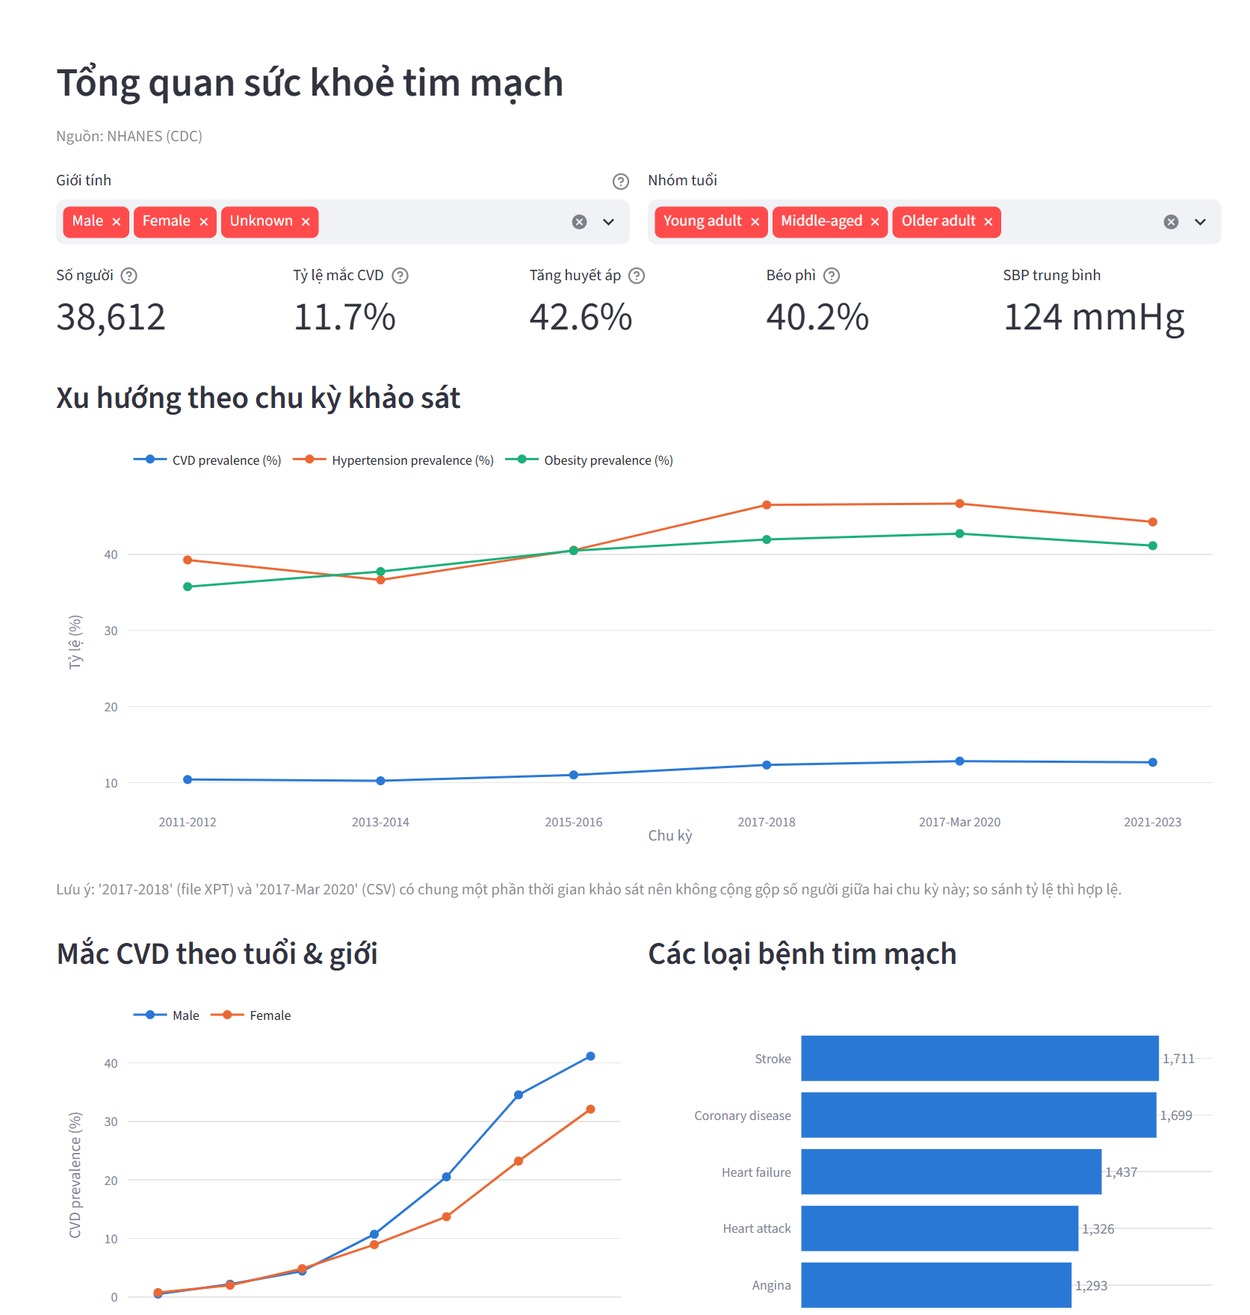
\includegraphics[width=0.7\textwidth]{figures/c_overview.png}
\caption{Trang Tổng quan}\label{fig:overview}
\end{figure}
Trang gồm năm thẻ KPI:
\begin{itemize}
\item Số người
\item Tỷ lệ mắc CVD
\item Tăng huyết áp
\item Béo phì
\item SBP trung bình
\end{itemize}
Ngoài ra trang có các biểu đồ:
\begin{itemize}
\item Xu hướng ba chỉ số (CVD, tăng huyết áp, béo phì) qua sáu chu kỳ khảo sát
\item Tỷ lệ CVD theo nhóm tuổi và giới tính
\item Số người theo từng loại bệnh tim mạch
\item Tỷ lệ CVD theo chủng tộc và theo mức thu nhập
\end{itemize}
Các biểu đồ cho phép nhanh chóng nhận ra xu hướng theo thời gian và các nhóm có tỷ lệ cao. Một số phát hiện chính: tỷ lệ CVD tăng khoảng 57 lần từ nhóm 20--29 tuổi (0,64\%) lên nhóm 80+ (36,35\%); nam cao hơn nữ (12,66\% so với 9,38\%); CVD tăng từ 10,4\% (2011--2012) lên 12,3\% (2017--2018), tăng huyết áp từ 39,3\% lên 46,5\%, béo phì từ 35,7\% lên 41,9\%; nhóm thu nhập cao nhất có tỷ lệ thấp nhất (7,00\%), nhóm thu nhập thấp có tỷ lệ cao nhất (14,12\%), tuy chưa hiệu chỉnh theo tuổi. Bộ lọc giới tính và nhóm tuổi áp dụng cho cả trang.

\section{Trang 2: OLAP Explorer}
Trang OLAP Explorer dành cho nhà phân tích muốn truy vấn đa chiều tự do mà không phải viết lại mã xử lý (câu hỏi Q2, Q9). Người dùng chọn chiều, thước đo và cách tổng hợp trên mô hình sao.
\begin{figure}[H]
\centering
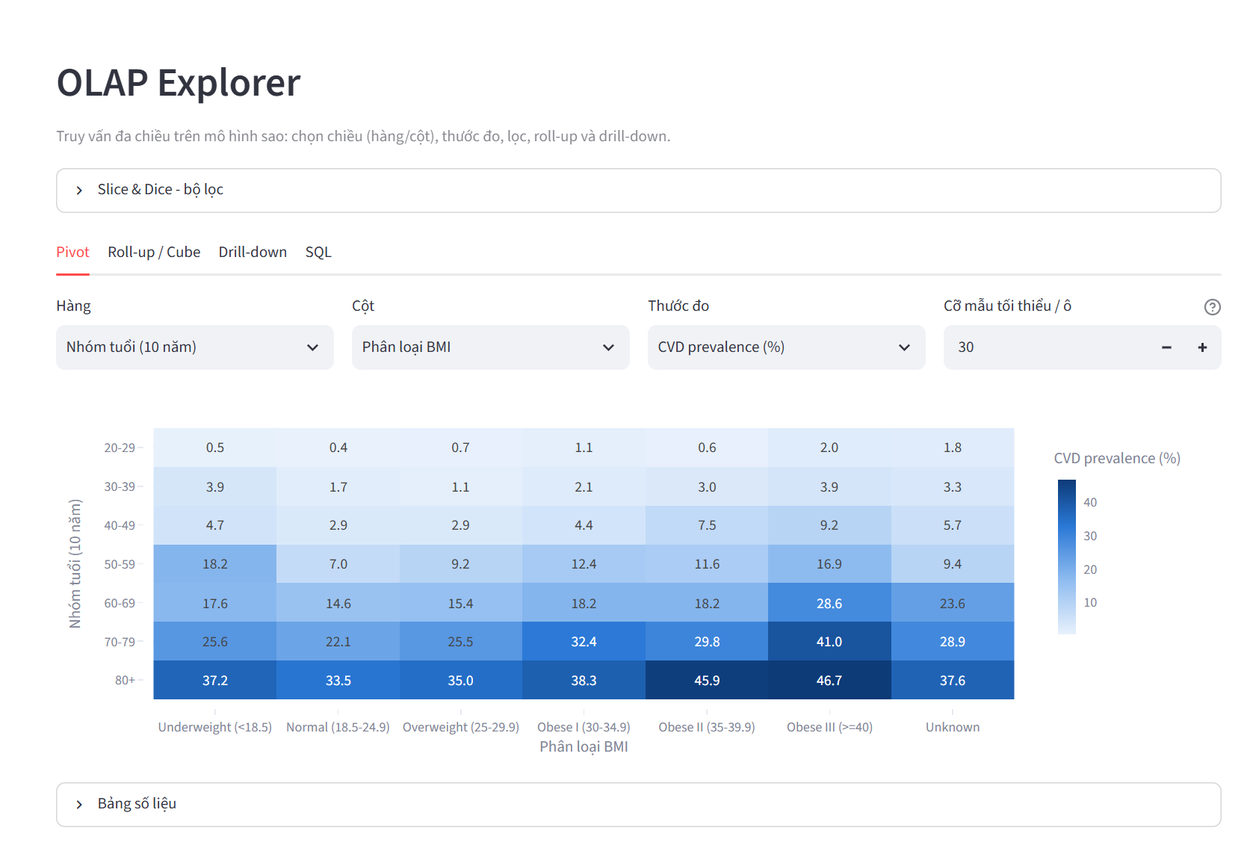
\includegraphics[width=0.7\textwidth]{figures/c_pivot.png}
\caption{OLAP Explorer -- Pivot: tỷ lệ CVD theo nhóm tuổi và phân loại BMI}\label{fig:pivot}
\end{figure}
Trang gồm bốn tab:
\begin{itemize}
\item \textbf{Pivot:} chọn chiều hàng, chiều cột, thước đo và cỡ mẫu tối thiểu mỗi ô; kết quả là bản đồ nhiệt.
\item \textbf{Roll-up / Cube:} bảng kết quả có dòng tổng phụ và tổng chung theo chế độ \emph{rollup}, \emph{cube} hoặc \emph{flat}; có nút tải CSV.
\item \textbf{Drill-down:} khoan từ mức thô xuống mức chi tiết của bảy phân cấp (Thời gian, Tuổi, Chủng tộc, Học vấn, Cân nặng, Huyết áp, Bệnh tim mạch).
\item \textbf{SQL:} ô truy vấn tự do, chỉ chấp nhận một câu \code{SELECT}/\code{WITH}.
\end{itemize}
Khung ``Slice \& Dice'' phía trên lọc theo chín chiều và áp dụng cho cả bốn tab. Các câu truy vấn tương ứng được cung cấp trong file \code{src/sql/truy_van_olap.sql}. Trang này giúp nhà phân tích trả lời nhanh các câu hỏi chưa có sẵn trên dashboard, đồng thời bảo đảm kết quả luôn nhất quán vì dùng chung một lớp truy vấn.

\section{Trang 3: Phân tích yếu tố nguy cơ}
Trang này giúp khám phá các yếu tố đằng sau sự chênh lệch giữa các nhóm (câu hỏi Q3--Q4). Vì tuổi chi phối mạnh nhất tỷ lệ CVD, trang so sánh các nhóm \emph{trong cùng nhóm tuổi} để tránh kết luận sai do khác biệt cấu trúc tuổi.
\begin{figure}[H]
\centering
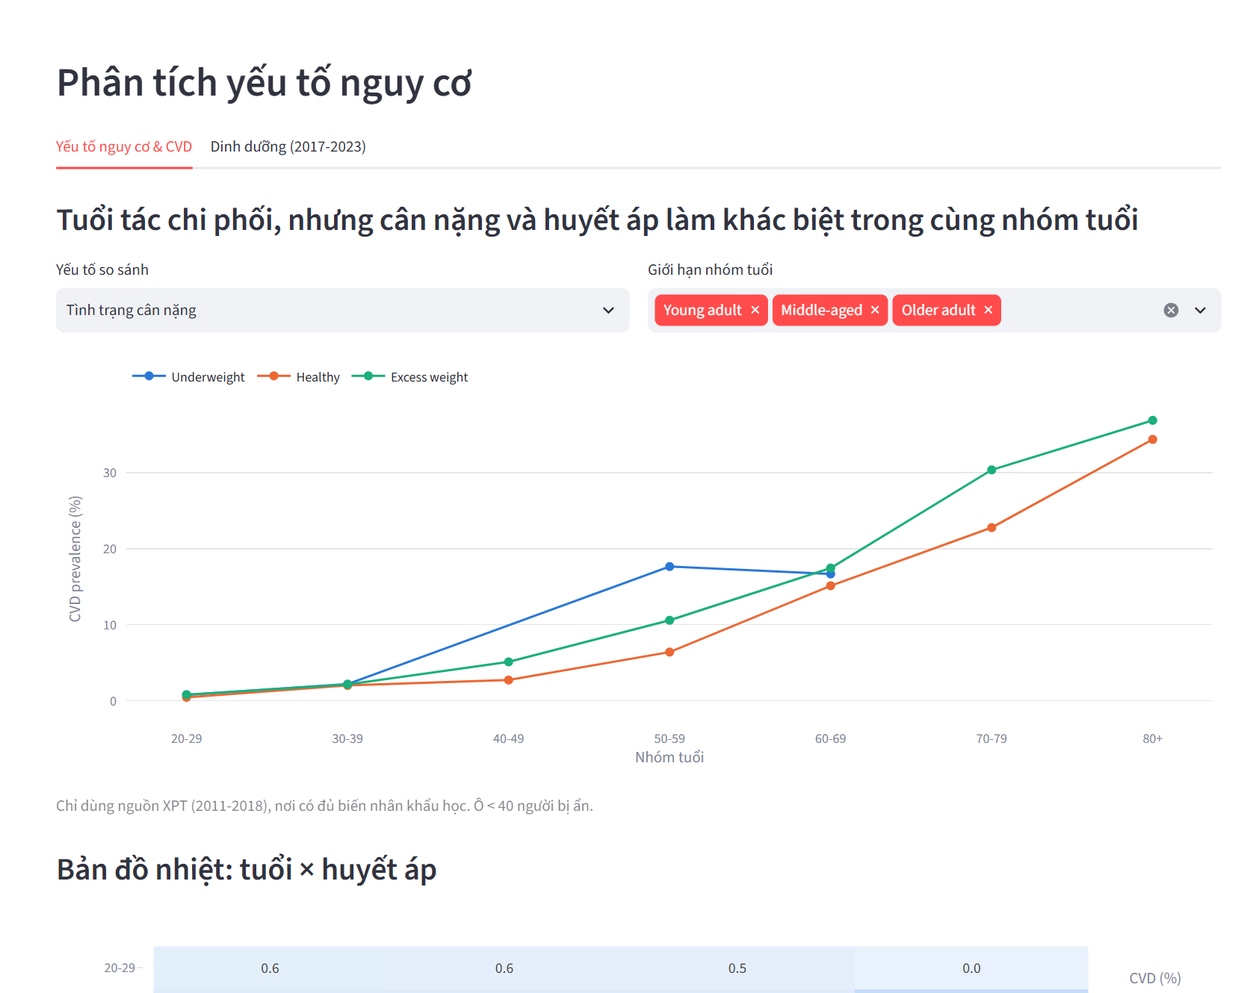
\includegraphics[width=0.7\textwidth]{figures/c_risk.png}
\caption{Trang Phân tích yếu tố nguy cơ}\label{fig:risk}
\end{figure}
Trang gồm hai tab:
\begin{itemize}
\item \textbf{Yếu tố nguy cơ \& CVD:} biểu đồ đường tỷ lệ CVD theo nhóm tuổi, tách theo một yếu tố được chọn (tình trạng cân nặng, nhóm huyết áp, cholesterol, thu nhập hoặc chủng tộc); bản đồ nhiệt nhóm tuổi $\times$ phân loại huyết áp.
\item \textbf{Dinh dưỡng:} so sánh khẩu phần (natri, kali, tỷ lệ Na/K, chất xơ, chất béo bão hòa, đường, cholesterol ăn vào) theo nhóm huyết áp, nhóm CVD, cân nặng, tuổi hoặc chu kỳ.
\end{itemize}
Ví dụ, ở nhóm 60--69 tuổi tỷ lệ CVD là 15,1\% ở người có BMI bình thường và 25,3\% ở người béo phì độ III. Về dinh dưỡng, trung bình mỗi người ăn 3.288 mg natri mỗi ngày; 68,8\% vượt ngưỡng khuyến nghị 2.300 mg và 83,8\% ăn dưới 25 g chất xơ. Trang kèm lưu ý diễn giải: dữ liệu cắt ngang, không có thông tin thuốc nên không suy ra nhân quả.

\section{Trang 4: Hệ hỗ trợ quyết định (DSS)}
Trang DSS dành cho lãnh đạo, chuyên viên chương trình và bác sĩ (câu hỏi Q5--Q8), gồm năm tab (nguyên lý ở Mục~3.7):
\begin{itemize}
\item \textbf{Nguy cơ cá nhân:} nhập tuổi, giới, huyết áp, BMI, cholesterol, HDL; nhận xác suất mắc CVD, mức nguy cơ, so sánh với nhóm cùng tuổi/giới, biểu đồ đóng góp của từng yếu tố và khuyến nghị theo màu (Hình~\ref{fig:individual}).
\item \textbf{What-if:} kéo ba thanh trượt (giảm huyết áp, cholesterol, BMI) và lọc nhóm dân số; xem nguy cơ trước/sau và số ca bệnh tránh được trên 1.000 người (Hình~\ref{fig:whatif}).
\item \textbf{Phân bổ ngân sách:} nhập dân số, chi phí mỗi người, ngân sách và tiêu chí phân khúc; xem xếp hạng phân khúc ưu tiên, độ phủ và so sánh với chia đều (Hình~\ref{fig:budget}).
\item \textbf{Cảnh báo xu hướng:} chọn chiều phân nhóm, chỉ báo và hai chu kỳ; xem biểu đồ thay đổi (cam = tăng, xanh = giảm, xám = ổn định) và bảng thống kê $z$.
\item \textbf{Mô hình:} cỡ mẫu huấn luyện/kiểm tra, AUC, Brier, đường hiệu chuẩn và lý do loại cholesterol, DBP khỏi mô hình.
\end{itemize}
\begin{figure}[H]
\centering
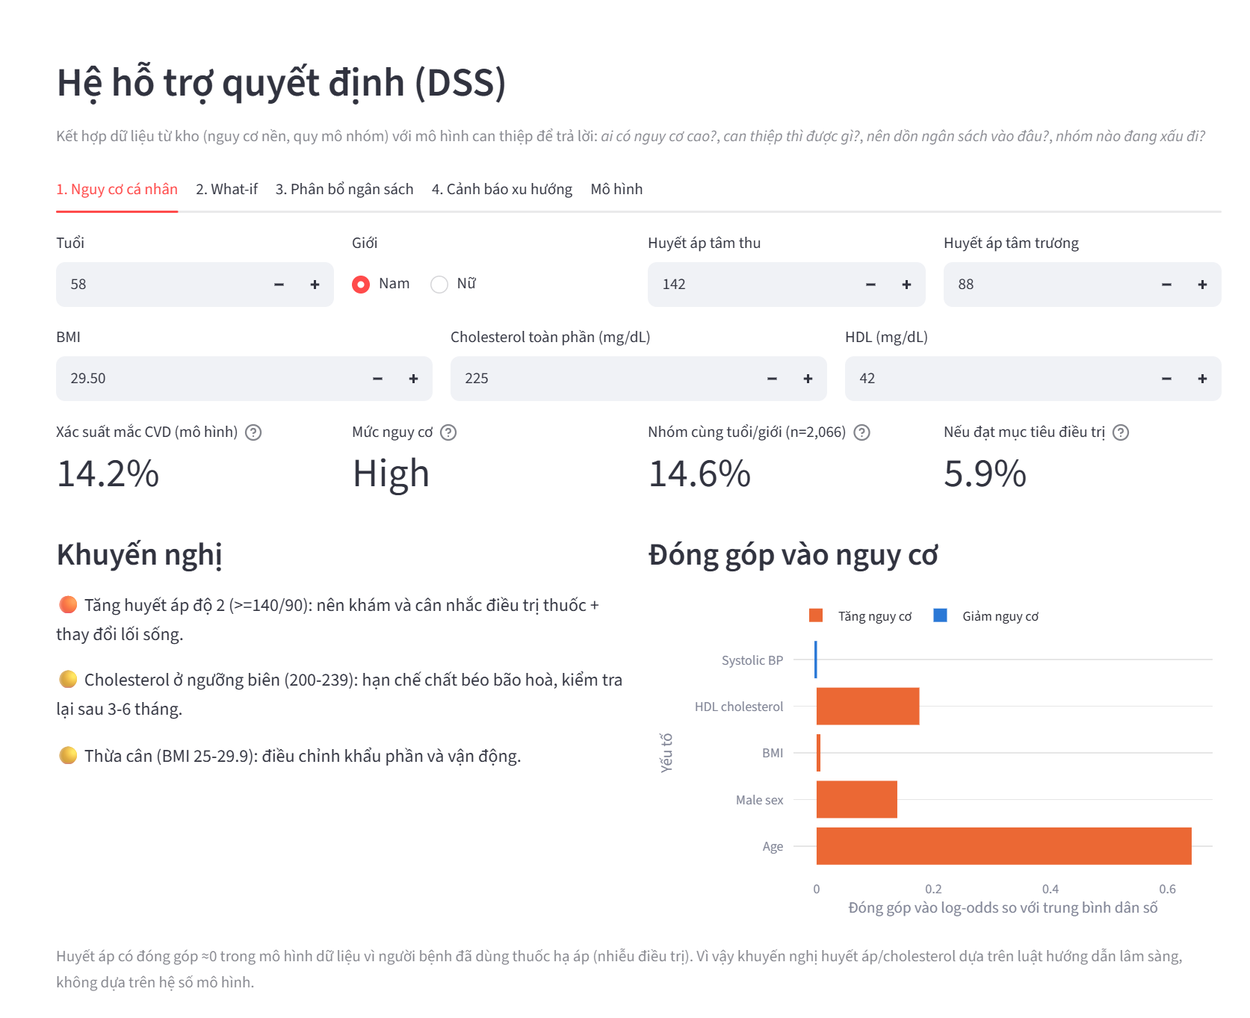
\includegraphics[width=0.62\textwidth]{figures/c_individual.png}
\caption{DSS -- Nguy cơ cá nhân}\label{fig:individual}
\end{figure}
\begin{figure}[H]
\centering
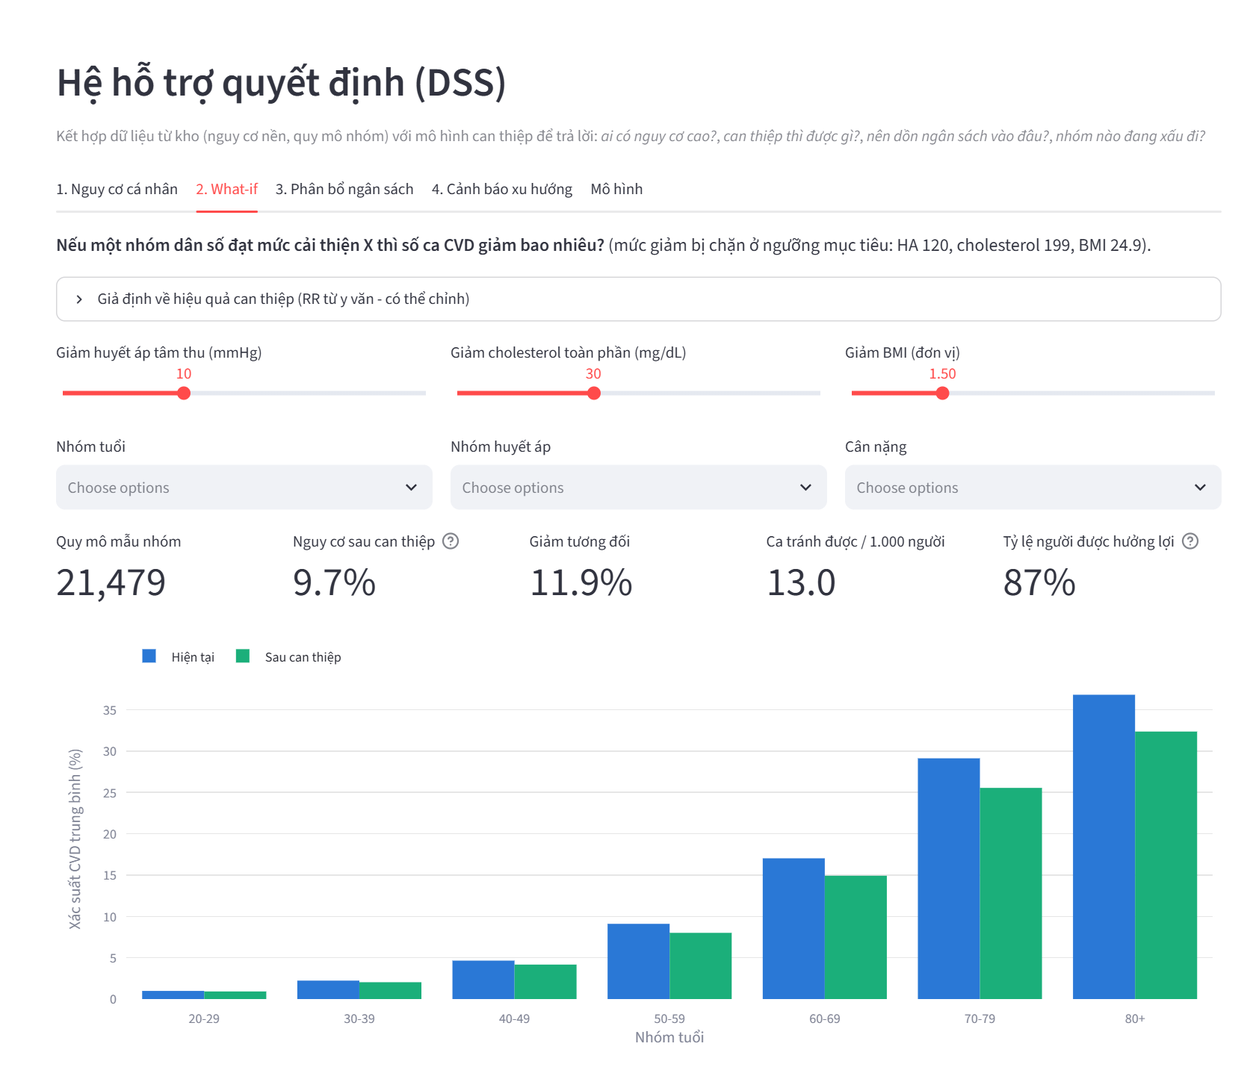
\includegraphics[width=0.62\textwidth]{figures/c_whatif.png}
\caption{DSS -- What-if}\label{fig:whatif}
\end{figure}
\begin{figure}[H]
\centering
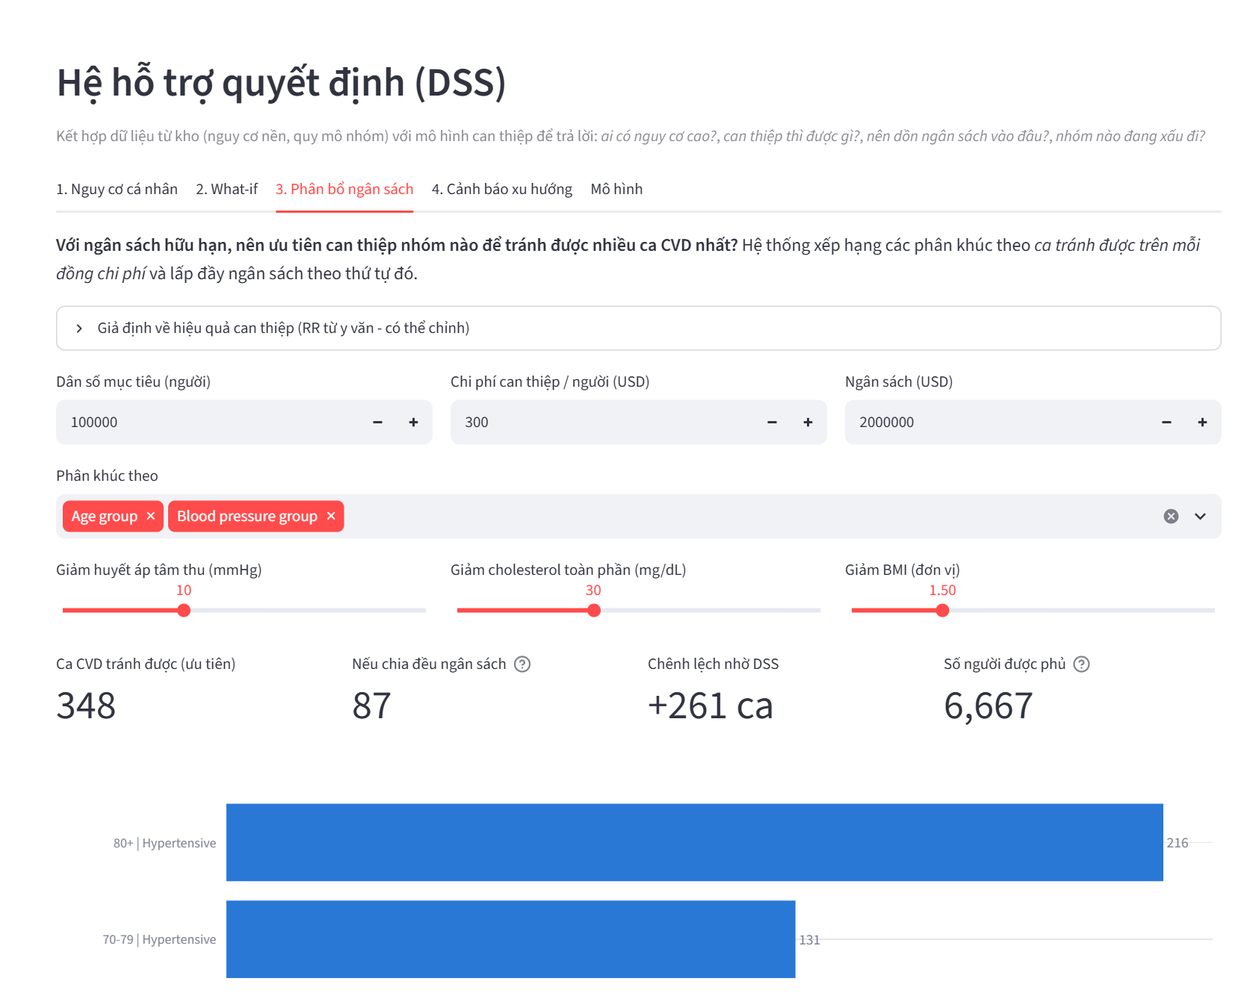
\includegraphics[width=0.62\textwidth]{figures/c_budget.png}
\caption{DSS -- Phân bổ ngân sách}\label{fig:budget}
\end{figure}

\section{Trang 5: Kho dữ liệu \& ETL}
Trang này dành cho nhà phân tích dữ liệu và người cần kiểm tra nguồn gốc số liệu (câu hỏi Q9). Trang gồm bốn tab: \emph{Sơ đồ sao} (sơ đồ và số dòng từng bảng, DDL), \emph{Nhật ký ETL} (số dòng Input, Output và Dropped của từng bước), \emph{Chất lượng dữ liệu} (độ đầy đủ theo chu kỳ, Hình~\ref{fig:dq}) và \emph{Từ điển dữ liệu} (định nghĩa các cờ và measure).
\begin{figure}[H]
\centering
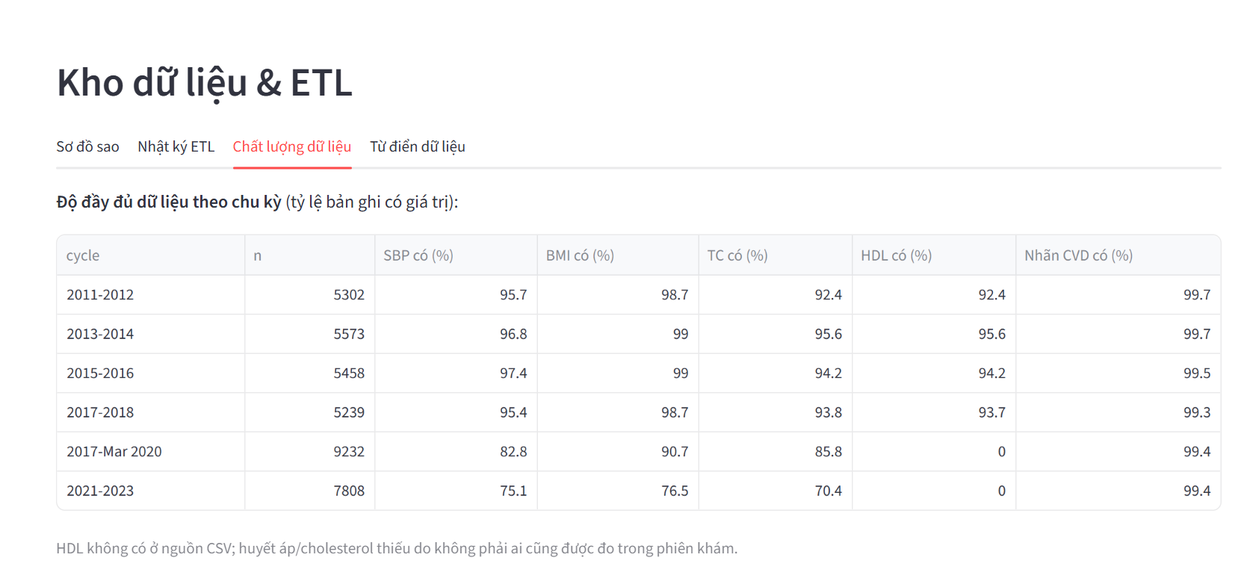
\includegraphics[width=0.7\textwidth]{figures/c_dq.png}
\caption{Trang Kho dữ liệu \& ETL -- độ đầy đủ dữ liệu theo chu kỳ}\label{fig:dq}
\end{figure}

\section{Tính tương tác}
Ứng dụng có các bộ lọc và điều khiển tương tác để phân tích linh hoạt. Các bộ lọc chính gồm:
\begin{itemize}
\item Giới tính và nhóm tuổi (trang Tổng quan)
\item Chu kỳ, giới tính, nhóm tuổi, nhóm chủng tộc, thu nhập, cân nặng, nhóm huyết áp, nhóm CVD, nguồn dữ liệu (khung Slice \& Dice của OLAP Explorer)
\item Yếu tố so sánh và giới hạn nhóm tuổi (trang Phân tích yếu tố nguy cơ)
\item Thanh trượt mức can thiệp, tham số hiệu quả, ngân sách và tiêu chí phân khúc (DSS)
\end{itemize}
Người dùng cũng có thể đặt cỡ mẫu tối thiểu để ẩn các ô quá nhỏ, tải kết quả dạng CSV và truy vấn SQL tự do.

Ứng dụng hỗ trợ một quy trình ra quyết định có cấu trúc:
\begin{enumerate}
\item \textbf{Tổng quan} -- theo dõi tình hình chung và xu hướng.
\item \textbf{OLAP Explorer} -- truy vấn và so sánh các nhóm theo nhiều chiều.
\item \textbf{Phân tích yếu tố nguy cơ} -- tìm yếu tố đằng sau chênh lệch.
\item \textbf{DSS} -- mô phỏng can thiệp, chọn nhóm ưu tiên, đánh giá cá nhân, cảnh báo xu hướng.
\item \textbf{Kho dữ liệu \& ETL} -- kiểm tra nguồn gốc và chất lượng số liệu.
\end{enumerate}
Dòng này giúp người dùng đi từ nhận định mức tổng quan đến phân tích chi tiết và quyết định cụ thể.

\section{Sự phù hợp với bài toán nghiệp vụ}
Ứng dụng giải quyết bài toán nghiệp vụ bằng cách biến các file khảo sát phân mảnh thành một ứng dụng phân tích tương tác. Thay vì phải ghép nối, làm sạch và tính lại số liệu thủ công cho mỗi câu hỏi, người dùng theo dõi chỉ số, so sánh các nhóm, mô phỏng can thiệp và chọn nhóm ưu tiên ngay trên giao diện. Ứng dụng phục vụ các nhóm người dùng khác nhau:
\begin{itemize}
\item \textbf{Lãnh đạo y tế công cộng} dùng trang Tổng quan và trang DSS (phân bổ ngân sách, cảnh báo xu hướng) để giám sát và quyết định ưu tiên.
\item \textbf{Chuyên viên chương trình} dùng what-if và phân bổ ngân sách để so sánh các phương án can thiệp.
\item \textbf{Nhà phân tích dữ liệu} dùng OLAP Explorer, trang Phân tích yếu tố nguy cơ và trang Kho dữ liệu \& ETL để truy vấn tự do và kiểm tra chất lượng.
\item \textbf{Bác sĩ phòng khám} dùng chức năng nguy cơ cá nhân để tư vấn từng người.
\end{itemize}
Việc cung cấp một giao diện tập trung và trực quan giúp tăng khả năng tiếp cận dữ liệu và hỗ trợ ra quyết định dựa trên bằng chứng.

\section{Tóm tắt}
Nhìn chung, ứng dụng đã phát triển cung cấp một công cụ BI và DSS thực tế cho phân tích nguy cơ bệnh tim mạch. Ứng dụng kết nối tới bảng phân tích đã làm sạch trong kho MySQL và trình bày dữ liệu qua năm trang: Tổng quan, OLAP Explorer, Phân tích yếu tố nguy cơ, DSS và Kho dữ liệu \& ETL. Ứng dụng giúp người quản lý theo dõi các chỉ số, so sánh và tìm nguyên nhân chênh lệch giữa các nhóm, mô phỏng can thiệp và chọn nhóm ưu tiên với ngân sách hữu hạn. Mặc dù dữ liệu hiện có giới hạn phạm vi ở tỷ lệ hiện mắc (không có thuốc, chi phí hay biến cố), ứng dụng vẫn chứng minh cách BI và các công nghệ liên quan biến dữ liệu khảo sát có cấu trúc thành thông tin hỗ trợ quyết định hữu ích.

\chapter{Đánh giá}\label{ch:eval}

\section{Tiêu chí đánh giá}
\begin{table}[H]
\renewcommand{\arraystretch}{1.35}\setlength{\extrarowheight}{3pt}
\centering
\caption{Đánh giá theo tiêu chí thành công đã đặt ra (Mục 2.4.2)}
\small
\begin{tabularx}{\textwidth}{|p{5.2cm}|X|p{1.7cm}|}
\hline
\textbf{Tiêu chí} & \textbf{Kết quả đo được} & \textbf{Đạt?} \\ \hline
Nạp từ nguồn thô bằng một lệnh, toàn vẹn khóa ngoại & ETL $\approx$ 25 giây; 16 khóa ngoại; kiểm thử không có khóa ngoại trỏ tới bản ghi không tồn tại (orphan), không trùng khóa & Đạt \\ \hline
Truy vấn tương tác dưới 1 giây & Qua bảng phẳng: 0,09--0,16 giây (trước tối ưu: 5,7--6,0 giây); cube 3 chiều $\approx$ 1,2 giây & Đạt (trừ cube nhiều chiều) \\ \hline
AUC $\geq$ 0,75 và Brier tốt hơn mô hình nền & AUC 0,794; Brier 0,0859 so với 0,0977 & Đạt \\ \hline
Trả lời ``ưu tiên nhóm nào'' trong $\leq$ 3 thao tác & Trang DSS: nhập ngân sách, chọn phân khúc, đọc xếp hạng & Đạt \\ \hline
Truy vết về nguồn & \code{etl_log} và trang Kho dữ liệu \& ETL; đối chiếu thủ công 4 bản ghi với file XPT gốc khớp hoàn toàn & Đạt \\ \hline
\end{tabularx}
\end{table}

\section{Kiểm thử tự động}
Bộ 15 kiểm thử (pytest) chạy trên MySQL thật, tất cả đạt: \emph{logic dimension} (3: ranh giới huyết áp ACC/AHA, nhóm BMI/tuổi, junk dimension); \emph{kho dữ liệu} (4: toàn vẹn tham chiếu 10 dimension, view và bảng phẳng không mất/nhân đôi dòng, \code{fact_nutrition} là tập con, giá trị trong khoảng sinh lý); \emph{OLAP} (4: tổng roll-up khớp, slice đúng và từ chối tên chiều độc hại, CVD tăng đơn điệu theo tuổi, drill-down khớp cha--con); \emph{DSS} (4: AUC, Brier và nguy cơ tăng theo tuổi; can thiệp không làm tăng nguy cơ và đơn điệu; phân bổ không vượt ngân sách và không kém chia đều; cảnh báo sắp xếp đúng). Năm trang dashboard (13 màn hình con) đã được mở trên trình duyệt thật và không có lỗi.

\section{Thành tựu}
\begin{itemize}
\item Kho dữ liệu đa chiều tích hợp hai nguồn NHANES: 38.612 bản ghi khám, 12.505 bản ghi dinh dưỡng, 10 dimension (5 dùng chung), 2 bảng fact, ETL có ghi nhật ký.
\item OLAP đầy đủ slice, dice, roll-up, drill-down, pivot, cube, cùng 22 truy vấn mẫu chạy được trên MySQL Workbench.
\item DSS bốn chức năng; trong kịch bản minh họa, ưu tiên đúng nhóm tránh được 348 ca so với 87 ca khi chia đều (cùng ngân sách, cùng 6.667 người được phủ).
\item Phát hiện và xử lý một vấn đề phương pháp quan trọng (nhiễu điều trị làm hệ số cholesterol sai dấu) bằng thiết kế thay vì che giấu.
\item Xử lý một nút thắt hiệu năng đặc thù của MySQL (lập kế hoạch join nhiều bảng) bằng bảng phẳng lưu sẵn.
\end{itemize}

\section{Hạn chế}\label{sec:limits}
\begin{itemize}
\item \textbf{Nhãn bệnh tự khai báo, cắt ngang:} mô hình ước lượng tỷ lệ hiện mắc, không dự báo biến cố và không chứng minh nhân quả.
\item \textbf{Nhiễu do điều trị chưa hiệu chỉnh:} hai nguồn không có dữ liệu thuốc nên huyết áp và cholesterol không đóng góp đúng chiều trong mô hình; tác động can thiệp dựa vào RR trong y văn (tham số BMI là giả định minh họa).
\item \textbf{Chưa gia quyền khảo sát và chưa chuẩn hóa tuổi:} tỷ lệ là tỷ lệ mẫu, không phải ước lượng cho toàn dân số; so sánh giữa chủng tộc, thu nhập chưa hiệu chỉnh tuổi; kiểm định $z$ chưa tính thiết kế mẫu phức hợp.
\item \textbf{Chu kỳ chồng lấn và thiếu thuộc tính:} ``2017--2018'' (nguồn A) chồng lấn ``2017--03/2020'' (nguồn B); nguồn B không có giới, chủng tộc, thu nhập nên bị loại khỏi các phân tích theo các chiều đó và khỏi huấn luyện mô hình.
\item \textbf{Quy mô và vận hành:} MySQL hướng hàng phù hợp quy mô hàng chục nghìn dòng; dữ liệu lớn hơn cần kho dạng cột/đám mây, nạp tăng dần, SCD; dashboard chưa có phân quyền người dùng.
\end{itemize}

\section{So sánh với mục tiêu}
\begin{table}[H]
\renewcommand{\arraystretch}{1.35}\setlength{\extrarowheight}{3pt}
\centering
\caption{Mức độ đạt các mục tiêu của dự án}
\small
\begin{tabularx}{\textwidth}{|X|p{2.2cm}|}
\hline
\textbf{Mục tiêu (Mục 2.4.1)} & \textbf{Mức độ} \\ \hline
Kho dữ liệu đa chiều tích hợp hai nguồn, ETL chạy lại được, có nhật ký & Hoàn thành \\ \hline
OLAP và dashboard trả lời Q1--Q4, Q9 & Hoàn thành \\ \hline
DSS trả lời Q5--Q8 dựa trên kho & Hoàn thành \\ \hline
Đánh giá trung thực, nêu giả định và hạn chế & Hoàn thành \\ \hline
\end{tabularx}
\end{table}

\chapter{Kết luận}\label{ch:conclusion}

\section{Tóm tắt}
Đề tài đã xây dựng hệ thống hoàn chỉnh từ dữ liệu thô đến quyết định: hai nguồn NHANES (24 file XPT và 1 file CSV, 2011--2023) được tích hợp bằng ETL có ghi nhật ký vào kho dữ liệu đa chiều MySQL (2 bảng fact, 10 dimension, 38.612 bản ghi khám và 12.505 bản ghi dinh dưỡng); tầng OLAP và dashboard cho phép khám phá đa chiều; và thành phần DSS với bốn chức năng -- đánh giá nguy cơ cá nhân, what-if, phân bổ ngân sách tối ưu, cảnh báo xu hướng -- trả lời câu hỏi cốt lõi: \emph{can thiệp vào nhóm dân số nào để tránh được nhiều ca bệnh tim mạch nhất với ngân sách hữu hạn}.

\section{Bài học kinh nghiệm}
\begin{itemize}
\item \textbf{Dữ liệu ``sạch'' vẫn cần giải mã:} phần lớn công sức ETL nằm ở việc hiểu mã hóa và quy ước (mã 7/9, huyết áp bằng 0, chu kỳ chồng lấn, trung bình các lần đo); sai ở tầng này lan ra mọi số liệu phía sau.
\item \textbf{Mô hình đúng thống kê chưa chắc dùng được:} mô hình bảy đặc trưng có AUC cao hơn nhưng hệ số cholesterol sai dấu y học; kiểm tra hệ số, không chỉ AUC, giúp tránh khuyến nghị sai.
\item \textbf{Hiệu năng phải đo, không đoán:} truy vấn chậm do lập kế hoạch join 11 bảng chứ không phải do thực thi; \code{EXPLAIN ANALYZE} và thí nghiệm chỉ ra giải pháp.
\item \textbf{Trung thực về giới hạn} (không nhân quả, không dự báo, chưa gia quyền) làm tăng độ tin cậy của hệ thống.
\end{itemize}

\section{Hướng phát triển}
\begin{enumerate}
\item \textbf{Hiệu chỉnh nhiễu do điều trị:} đưa bảng thuốc, tiểu đường, hút thuốc từ bộ NHANES 2013--2014 dạng rộng vào kho (thêm dimension) để mô hình dùng được huyết áp và cholesterol đúng chiều.
\item \textbf{Gia quyền khảo sát và chuẩn hóa tuổi:} dùng \code{mec_weight} và cụm/tầng mẫu để ước lượng tỷ lệ và khoảng tin cậy cho toàn dân số.
\item \textbf{Dự báo biến cố:} liên kết dữ liệu tử vong (NHANES Linked Mortality) để mô hình theo thời gian thay cho hiện mắc.
\item \textbf{Tối ưu mạnh hơn:} nhiều ràng buộc (nhân lực, độ phủ tối thiểu vì công bằng), đa mục tiêu, phân tích độ nhạy tự động theo tham số RR.
\item \textbf{Kiến trúc và vận hành:} vùng staging trong CSDL, nạp tăng dần, SCD; kho dạng cột (ClickHouse, BigQuery) khi dữ liệu lớn; phân quyền, tài khoản chỉ đọc riêng, lập lịch ETL.
\end{enumerate}

\begin{thebibliography}{99}
\bibitem{kimball2013} R. Kimball, M. Ross, \emph{The Data Warehouse Toolkit}, 3rd ed., Wiley, 2013.
\bibitem{inmon2005} W. H. Inmon, \emph{Building the Data Warehouse}, 4th ed., Wiley, 2005.
\bibitem{turban2005} E. Turban, J. E. Aronson, T.-P. Liang, \emph{Decision Support Systems and Intelligent Systems}, 7th ed., Prentice-Hall, 2005.
\bibitem{sharda2020} R. Sharda, D. Delen, E. Turban, \emph{Analytics, Data Science, \& Artificial Intelligence: Systems for Decision Support}, 11th ed., Pearson, 2020.
\bibitem{han2012} J. Han, M. Kamber, J. Pei, \emph{Data Mining: Concepts and Techniques}, 3rd ed., Morgan Kaufmann, 2012.
\bibitem{simon1960} H. A. Simon, \emph{The New Science of Management Decision}, Harper \& Row, 1960.
\bibitem{nhanes} CDC, National Center for Health Statistics, \emph{National Health and Nutrition Examination Survey (NHANES)}. \texttt{https://www.cdc.gov/nchs/nhanes/}
\bibitem{who_cvd} World Health Organization, \emph{Cardiovascular diseases (CVDs) -- fact sheet}. \texttt{https://www.who.int/news-room/fact-sheets/detail/cardiovascular-diseases-(cvds)}
\bibitem{acc_aha2017} P. K. Whelton et al., 2017 ACC/AHA guideline for the prevention, detection, evaluation, and management of high blood pressure in adults, \emph{Hypertension}, 71(6), e13--e115, 2018.
\bibitem{atp3} National Cholesterol Education Program, Third Report of the Expert Panel on Detection, Evaluation, and Treatment of High Blood Cholesterol in Adults (ATP III), \emph{Circulation}, 106, 3143--3421, 2002.
\bibitem{ettehad2016} D. Ettehad et al., Blood pressure lowering for prevention of cardiovascular disease and death: a systematic review and meta-analysis, \emph{The Lancet}, 387, 957--967, 2016.
\bibitem{ctt2010} Cholesterol Treatment Trialists' (CTT) Collaboration, Efficacy and safety of more intensive lowering of LDL cholesterol: a meta-analysis of data from 170\,000 participants in 26 randomised trials, \emph{The Lancet}, 376, 1670--1681, 2010.
\bibitem{erfc2011} Emerging Risk Factors Collaboration, Separate and combined associations of body-mass index and abdominal adiposity with cardiovascular disease: collaborative analysis of 58 prospective studies, \emph{The Lancet}, 377, 1085--1096, 2011.
\end{thebibliography}

\end{document}
